\documentclass[1p]{elsarticle_modified}
%\bibliographystyle{elsarticle-num}

%\usepackage[colorlinks]{hyperref}
%\usepackage{abbrmath_seonhwa} %\Abb, \Ascr, \Acal ,\Abf, \Afrak
\usepackage{amsfonts}
\usepackage{amssymb}
\usepackage{amsmath}
\usepackage{amsthm}
\usepackage{scalefnt}
\usepackage{amsbsy}
\usepackage{kotex}
\usepackage{caption}
\usepackage{subfig}
\usepackage{color}
\usepackage{graphicx}
\usepackage{xcolor} %% white, black, red, green, blue, cyan, magenta, yellow
\usepackage{float}
\usepackage{setspace}
\usepackage{hyperref}

\usepackage{tikz}
\usetikzlibrary{arrows}

\usepackage{multirow}
\usepackage{array} % fixed length table
\usepackage{hhline}

%%%%%%%%%%%%%%%%%%%%%
\makeatletter
\renewcommand*\env@matrix[1][\arraystretch]{%
	\edef\arraystretch{#1}%
	\hskip -\arraycolsep
	\let\@ifnextchar\new@ifnextchar
	\array{*\c@MaxMatrixCols c}}
\makeatother %https://tex.stackexchange.com/questions/14071/how-can-i-increase-the-line-spacing-in-a-matrix
%%%%%%%%%%%%%%%

\usepackage[normalem]{ulem}

\newcommand{\msout}[1]{\ifmmode\text{\sout{\ensuremath{#1}}}\else\sout{#1}\fi}
%SOURCE: \msout is \stkout macro in https://tex.stackexchange.com/questions/20609/strikeout-in-math-mode

\newcommand{\cancel}[1]{
	\ifmmode
	{\color{red}\msout{#1}}
	\else
	{\color{red}\sout{#1}}
	\fi
}

\newcommand{\add}[1]{
	{\color{blue}\uwave{#1}}
}

\newcommand{\replace}[2]{
	\ifmmode
	{\color{red}\msout{#1}}{\color{blue}\uwave{#2}}
	\else
	{\color{red}\sout{#1}}{\color{blue}\uwave{#2}}
	\fi
}

\newcommand{\Sol}{\mathcal{S}} %segment
\newcommand{\D}{D} %diagram
\newcommand{\A}{\mathcal{A}} %arc


%%%%%%%%%%%%%%%%%%%%%%%%%%%%%5 test

\def\sl{\operatorname{\textup{SL}}(2,\Cbb)}
\def\psl{\operatorname{\textup{PSL}}(2,\Cbb)}
\def\quan{\mkern 1mu \triangleright \mkern 1mu}

\theoremstyle{definition}
\newtheorem{thm}{Theorem}[section]
\newtheorem{prop}[thm]{Proposition}
\newtheorem{lem}[thm]{Lemma}
\newtheorem{ques}[thm]{Question}
\newtheorem{cor}[thm]{Corollary}
\newtheorem{defn}[thm]{Definition}
\newtheorem{exam}[thm]{Example}
\newtheorem{rmk}[thm]{Remark}
\newtheorem{alg}[thm]{Algorithm}

\newcommand{\I}{\sqrt{-1}}
\begin{document}

%\begin{frontmatter}
%
%\title{Boundary parabolic representations of knots up to 8 crossings}
%
%%% Group authors per affiliation:
%\author{Yunhi Cho} 
%\address{Department of Mathematics, University of Seoul, Seoul, Korea}
%\ead{yhcho@uos.ac.kr}
%
%
%\author{Seonhwa Kim} %\fnref{s_kim}}
%\address{Center for Geometry and Physics, Institute for Basic Science, Pohang, 37673, Korea}
%\ead{ryeona17@ibs.re.kr}
%
%\author{Hyuk Kim}
%\address{Department of Mathematical Sciences, Seoul National University, Seoul 08826, Korea}
%\ead{hyukkim@snu.ac.kr}
%
%\author{Seokbeom Yoon}
%\address{Department of Mathematical Sciences, Seoul National University, Seoul, 08826,  Korea}
%\ead{sbyoon15@snu.ac.kr}
%
%\begin{abstract}
%We find all boundary parabolic representation of knots up to 8 crossings.
%
%\end{abstract}
%\begin{keyword}
%    \MSC[2010] 57M25 
%\end{keyword}
%
%\end{frontmatter}

%\linenumbers
%\tableofcontents
%
\newcommand\colored[1]{\textcolor{white}{\rule[-0.35ex]{0.8em}{1.4ex}}\kern-0.8em\color{red} #1}%
%\newcommand\colored[1]{\textcolor{white}{ #1}\kern-2.17ex	\textcolor{white}{ #1}\kern-1.81ex	\textcolor{white}{ #1}\kern-2.15ex\color{red}#1	}

{\Large $\underline{12a_{1022}~(K12a_{1022})}$}

\setlength{\tabcolsep}{10pt}
\renewcommand{\arraystretch}{1.6}
\vspace{1cm}\begin{tabular}{m{100pt}>{\centering\arraybackslash}m{274pt}}
\multirow{5}{120pt}{
	\centering
	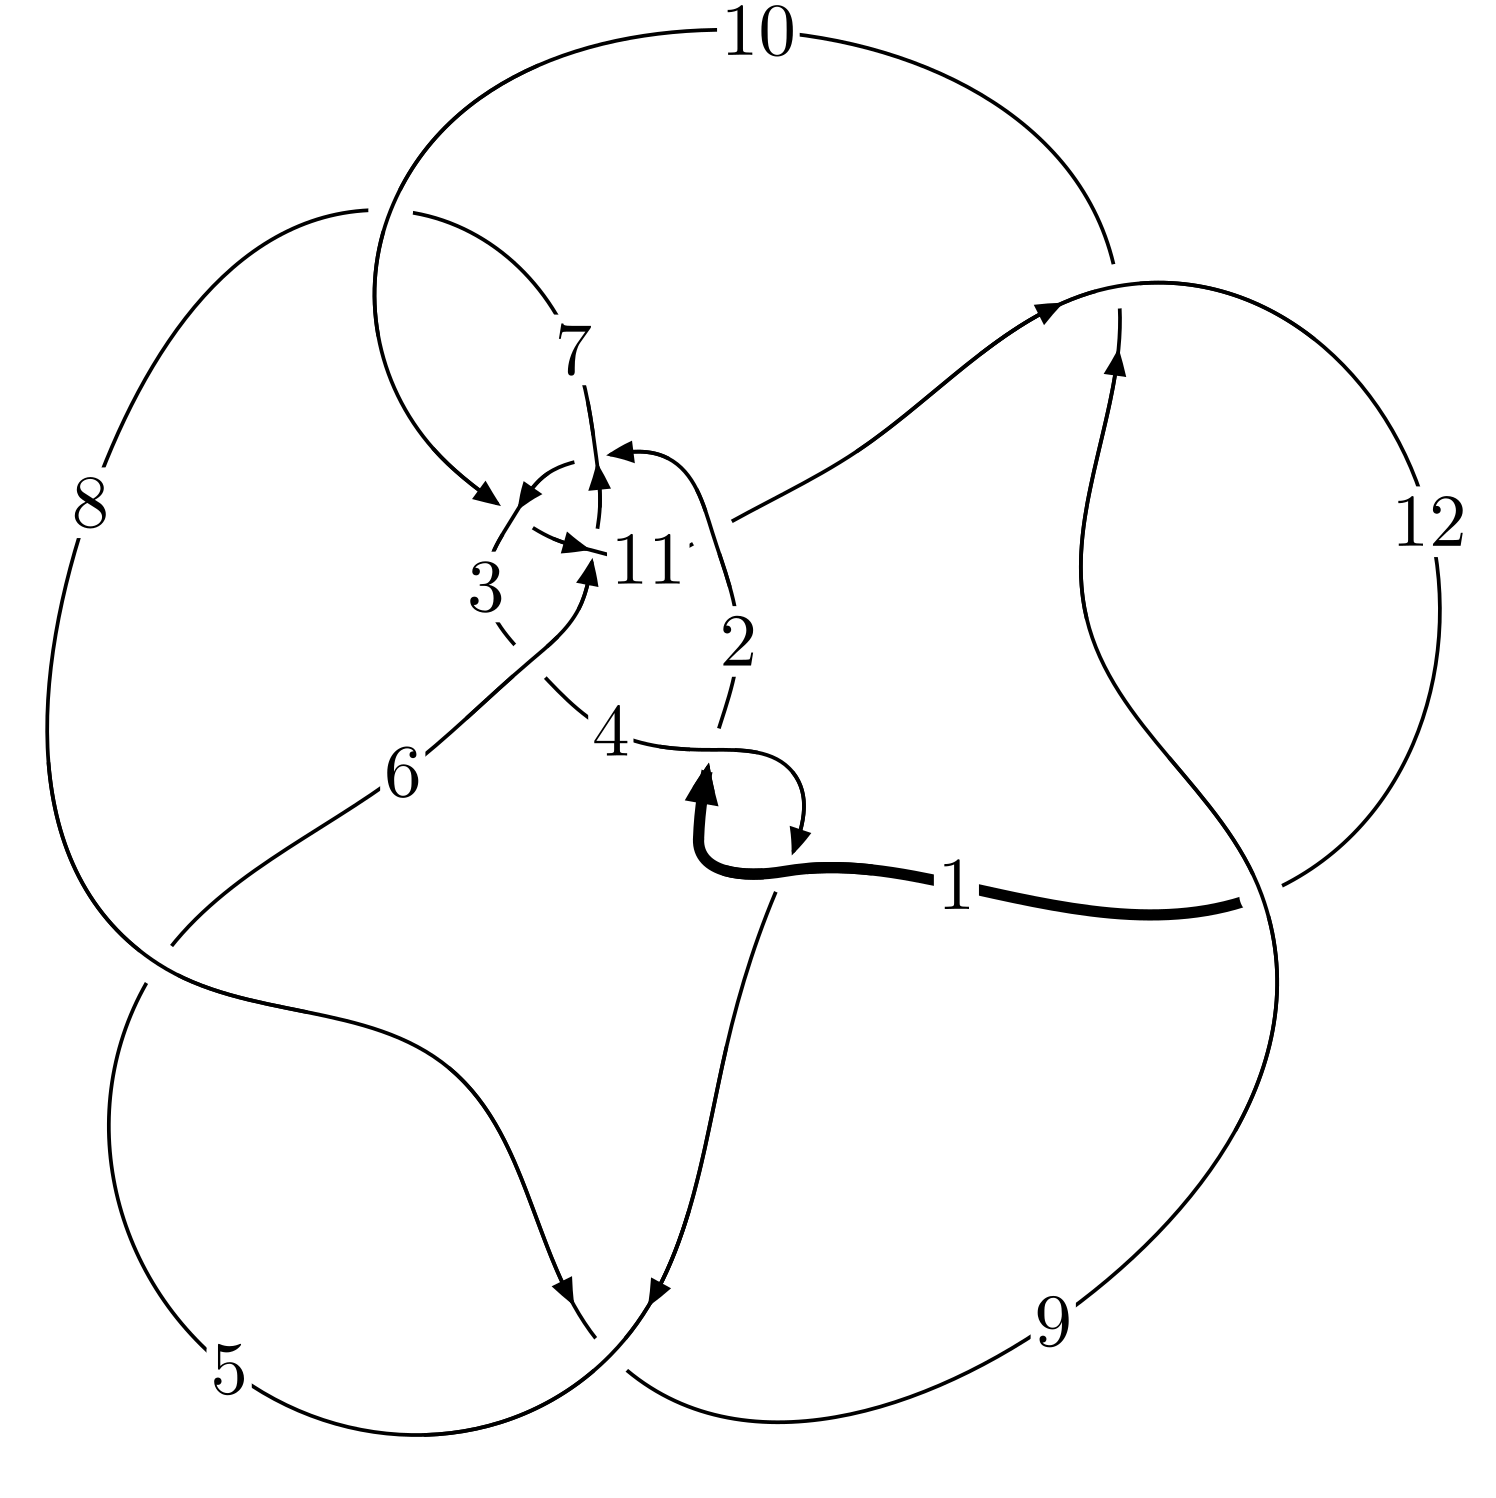
\includegraphics[width=112pt]{../../../GIT/diagram.site/Diagrams/png/1823_12a_1022.png}\\
\ \ \ A knot diagram\footnotemark}&
\allowdisplaybreaks
\textbf{Linearized knot diagam} \\
\cline{2-2}
 &
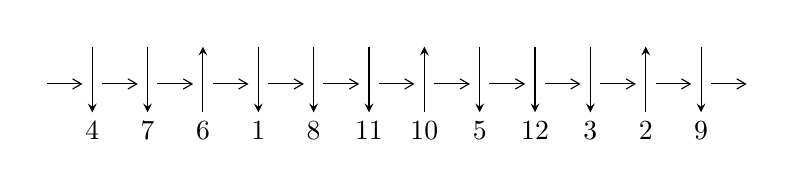
\begin{tikzpicture}[x=20pt, y=17pt]
	% nodes
	\node (C0) at (0, 0) {};
	\node (C1) at (1, 0) {};
	\node (C1U) at (1, +1) {};
	\node (C1D) at (1, -1) {4};

	\node (C2) at (2, 0) {};
	\node (C2U) at (2, +1) {};
	\node (C2D) at (2, -1) {7};

	\node (C3) at (3, 0) {};
	\node (C3U) at (3, +1) {};
	\node (C3D) at (3, -1) {6};

	\node (C4) at (4, 0) {};
	\node (C4U) at (4, +1) {};
	\node (C4D) at (4, -1) {1};

	\node (C5) at (5, 0) {};
	\node (C5U) at (5, +1) {};
	\node (C5D) at (5, -1) {8};

	\node (C6) at (6, 0) {};
	\node (C6U) at (6, +1) {};
	\node (C6D) at (6, -1) {11};

	\node (C7) at (7, 0) {};
	\node (C7U) at (7, +1) {};
	\node (C7D) at (7, -1) {10};

	\node (C8) at (8, 0) {};
	\node (C8U) at (8, +1) {};
	\node (C8D) at (8, -1) {5};

	\node (C9) at (9, 0) {};
	\node (C9U) at (9, +1) {};
	\node (C9D) at (9, -1) {12};

	\node (C10) at (10, 0) {};
	\node (C10U) at (10, +1) {};
	\node (C10D) at (10, -1) {3};

	\node (C11) at (11, 0) {};
	\node (C11U) at (11, +1) {};
	\node (C11D) at (11, -1) {2};

	\node (C12) at (12, 0) {};
	\node (C12U) at (12, +1) {};
	\node (C12D) at (12, -1) {9};
	\node (C13) at (13, 0) {};

	% arrows
	\draw[->,>={angle 60}]
	(C0) edge (C1) (C1) edge (C2) (C2) edge (C3) (C3) edge (C4) (C4) edge (C5) (C5) edge (C6) (C6) edge (C7) (C7) edge (C8) (C8) edge (C9) (C9) edge (C10) (C10) edge (C11) (C11) edge (C12) (C12) edge (C13) ;	\draw[->,>=stealth]
	(C1U) edge (C1D) (C2U) edge (C2D) (C3D) edge (C3U) (C4U) edge (C4D) (C5U) edge (C5D) (C6U) edge (C6D) (C7D) edge (C7U) (C8U) edge (C8D) (C9U) edge (C9D) (C10U) edge (C10D) (C11D) edge (C11U) (C12U) edge (C12D) ;
	\end{tikzpicture} \\
\hhline{~~} \\& 
\textbf{Solving Sequence} \\ \cline{2-2} 
 &
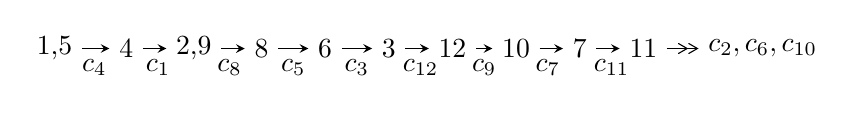
\begin{tikzpicture}[x=23pt, y=7pt]
	% node
	\node (A0) at (-1/8, 0) {1,5};
	\node (A1) at (1, 0) {4};
	\node (A2) at (33/16, 0) {2,9};
	\node (A3) at (25/8, 0) {8};
	\node (A4) at (33/8, 0) {6};
	\node (A5) at (41/8, 0) {3};
	\node (A6) at (49/8, 0) {12};
	\node (A7) at (57/8, 0) {10};
	\node (A8) at (65/8, 0) {7};
	\node (A9) at (73/8, 0) {11};
	\node (C1) at (1/2, -1) {$c_{4}$};
	\node (C2) at (3/2, -1) {$c_{1}$};
	\node (C3) at (21/8, -1) {$c_{8}$};
	\node (C4) at (29/8, -1) {$c_{5}$};
	\node (C5) at (37/8, -1) {$c_{3}$};
	\node (C6) at (45/8, -1) {$c_{12}$};
	\node (C7) at (53/8, -1) {$c_{9}$};
	\node (C8) at (61/8, -1) {$c_{7}$};
	\node (C9) at (69/8, -1) {$c_{11}$};
	\node (A10) at (11, 0) {$c_{2},c_{6},c_{10}$};

	% edge
	\draw[->,>=stealth]	
	(A0) edge (A1) (A1) edge (A2) (A2) edge (A3) (A3) edge (A4) (A4) edge (A5) (A5) edge (A6) (A6) edge (A7) (A7) edge (A8) (A8) edge (A9) ;
	\draw[->>,>={angle 60}]	
	(A9) edge (A10);
\end{tikzpicture} \\ 

\end{tabular} \\

\footnotetext{
The image of knot diagram is generated by the software ``\textbf{Draw programme}" developed by Andrew Bartholomew(\url{http://www.layer8.co.uk/maths/draw/index.htm\#Running-draw}), where we modified some parts for our purpose(\url{https://github.com/CATsTAILs/LinksPainter}).
}\phantom \\ \newline 
\centering \textbf{Ideals for irreducible components\footnotemark of $X_{\text{par}}$} 
 
\begin{align*}
I^u_{1}&=\langle 
b- u,\;a-1,\;u^{11}+3 u^{10}+10 u^9+16 u^8+25 u^7+22 u^6+17 u^5+7 u^4+2 u^3+2 u^2+2 u-1\rangle \\
I^u_{2}&=\langle 
b- u,\;-32833783 u^{25}+115127419 u^{24}+\cdots+15217558 a+63920326,\;u^{26}-4 u^{25}+\cdots-8 u+1\rangle \\
I^u_{3}&=\langle 
-16207713 u^{25}+59026143 u^{24}+\cdots+15217558 b+32833783,\;a-1,\;u^{26}-4 u^{25}+\cdots-8 u+1\rangle \\
I^u_{4}&=\langle 
-1.98504\times10^{21} u^{25}-3.05841\times10^{22} u^{24}+\cdots+4.27582\times10^{21} b-1.24580\times10^{24},\\
\phantom{I^u_{4}}&\phantom{= \langle  }7.78622\times10^{22} u^{25}+1.18227\times10^{24} u^{24}+\cdots+1.36826\times10^{23} a+2.49940\times10^{25},\\
\phantom{I^u_{4}}&\phantom{= \langle  }u^{26}+16 u^{25}+\cdots+4800 u+512\rangle \\
I^u_{5}&=\langle 
b+u,\;a+1,\;u^{10}+2 u^9+6 u^8+6 u^7+9 u^6+5 u^5+6 u^4+3 u^3+3 u^2+u+1\rangle \\
I^u_{6}&=\langle 
b+u,\;2 u^9+u^8+10 u^7+8 u^6+22 u^5+19 u^4+25 u^3+17 u^2+a+13 u+3,\\
\phantom{I^u_{6}}&\phantom{= \langle  }u^{10}+u^9+5 u^8+6 u^7+12 u^6+13 u^5+15 u^4+12 u^3+9 u^2+4 u+1\rangle \\
I^u_{7}&=\langle 
- u^9-4 u^7-2 u^6-7 u^5-5 u^4-7 u^3-5 u^2+b-5 u-2,\;a+1,\\
\phantom{I^u_{7}}&\phantom{= \langle  }u^{10}+u^9+5 u^8+6 u^7+12 u^6+13 u^5+15 u^4+12 u^3+9 u^2+4 u+1\rangle \\
I^u_{8}&=\langle 
136 u^9+138 u^8+938 u^7+182 u^6+237 u^5-1628 u^4-2106 u^3-2845 u^2+809 b-2290 u-883,\\
\phantom{I^u_{8}}&\phantom{= \langle  }883 u^9+3668 u^8+\cdots+809 a+2125,\\
\phantom{I^u_{8}}&\phantom{= \langle  }u^{10}+4 u^9+15 u^8+34 u^7+57 u^6+71 u^5+66 u^4+45 u^3+20 u^2+5 u+1\rangle \\
I^u_{9}&=\langle 
-3.23739\times10^{22} u^{35}+2.81046\times10^{23} u^{34}+\cdots+6.80585\times10^{22} b+8.32842\times10^{23},\\
\phantom{I^u_{9}}&\phantom{= \langle  }-2.58181\times10^{25} a u^{35}-1.04570\times10^{25} u^{35}+\cdots+6.94260\times10^{26} a-5.64319\times10^{26},\\
\phantom{I^u_{9}}&\phantom{= \langle  }u^{36}-9 u^{35}+\cdots-134 u+31\rangle \\
\\
\end{align*}
\raggedright * 9 irreducible components of $\dim_{\mathbb{C}}=0$, with total 201 representations.\\
\footnotetext{All coefficients of polynomials are rational numbers. But the coefficients are sometimes approximated in decimal forms when there is not enough margin.}
\newpage
\renewcommand{\arraystretch}{1}
\centering \section*{I. $I^u_{1}= \langle b- u,\;a-1,\;u^{11}+3 u^{10}+\cdots+2 u-1 \rangle$}
\flushleft \textbf{(i) Arc colorings}\\
\begin{tabular}{m{7pt} m{180pt} m{7pt} m{180pt} }
\flushright $a_{1}=$&$\begin{pmatrix}0\\u\end{pmatrix}$ \\
\flushright $a_{5}=$&$\begin{pmatrix}1\\0\end{pmatrix}$ \\
\flushright $a_{4}=$&$\begin{pmatrix}1\\- u^2\end{pmatrix}$ \\
\flushright $a_{2}=$&$\begin{pmatrix}- u\\u^3+u\end{pmatrix}$ \\
\flushright $a_{9}=$&$\begin{pmatrix}1\\u\end{pmatrix}$ \\
\flushright $a_{8}=$&$\begin{pmatrix}u+1\\u\end{pmatrix}$ \\
\flushright $a_{6}=$&$\begin{pmatrix}u^2+u+1\\u^2\end{pmatrix}$ \\
\flushright $a_{3}=$&$\begin{pmatrix}u^6+2 u^5+4 u^4+3 u^3+2 u^2+1\\u^6+u^5+2 u^4- u^2\end{pmatrix}$ \\
\flushright $a_{12}=$&$\begin{pmatrix}u\\u^2+u\end{pmatrix}$ \\
\flushright $a_{10}=$&$\begin{pmatrix}u^2+1\\u^3+u^2+u\end{pmatrix}$ \\
\flushright $a_{7}=$&$\begin{pmatrix}u^6+u^5+3 u^4+u^3+2 u^2+u+1\\u^7+2 u^6+4 u^5+3 u^4+2 u^3+u\end{pmatrix}$ \\
\flushright $a_{11}=$&$\begin{pmatrix}- u^5- u^4-2 u^3+u\\u^7+u^6+3 u^5+u^4+2 u^3+u^2+u\end{pmatrix}$\\&\end{tabular}
\flushleft \textbf{(ii) Obstruction class $= -1$}\\~\\
\flushleft \textbf{(iii) Cusp Shapes $= -3 u^{10}-9 u^9-27 u^8-45 u^7-63 u^6-63 u^5-45 u^4-24 u^3-12 u^2-9$}\\~\\
\newpage\renewcommand{\arraystretch}{1}
\flushleft \textbf{(iv) u-Polynomials at the component}\newline \\
\begin{tabular}{m{50pt}|m{274pt}}
Crossings & \hspace{64pt}u-Polynomials at each crossing \\
\hline $$\begin{aligned}c_{1},c_{4},c_{5}\\c_{8},c_{9},c_{12}\end{aligned}$$&$\begin{aligned}
&u^{11}-3 u^{10}+\cdots+2 u+1
\end{aligned}$\\
\hline $$\begin{aligned}c_{2},c_{6},c_{10}\end{aligned}$$&$\begin{aligned}
&u^{11}+5 u^{10}+13 u^9+20 u^8+21 u^7+15 u^6+9 u^5+4 u^4+2 u^3+u+1
\end{aligned}$\\
\hline $$\begin{aligned}c_{3},c_{7},c_{11}\end{aligned}$$&$\begin{aligned}
&u^{11}+6 u^{10}+\cdots+13 u+2
\end{aligned}$\\
\hline
\end{tabular}\\~\\
\newpage\renewcommand{\arraystretch}{1}
\flushleft \textbf{(v) Riley Polynomials at the component}\newline \\
\begin{tabular}{m{50pt}|m{274pt}}
Crossings & \hspace{64pt}Riley Polynomials at each crossing \\
\hline $$\begin{aligned}c_{1},c_{4},c_{5}\\c_{8},c_{9},c_{12}\end{aligned}$$&$\begin{aligned}
&y^{11}+11 y^{10}+\cdots+8 y-1
\end{aligned}$\\
\hline $$\begin{aligned}c_{2},c_{6},c_{10}\end{aligned}$$&$\begin{aligned}
&y^{11}+y^{10}+\cdots+y-1
\end{aligned}$\\
\hline $$\begin{aligned}c_{3},c_{7},c_{11}\end{aligned}$$&$\begin{aligned}
&y^{11}+2 y^{10}+\cdots+73 y-4
\end{aligned}$\\
\hline
\end{tabular}\\~\\
\newpage\flushleft \textbf{(vi) Complex Volumes and Cusp Shapes}
$$\begin{array}{c|c|c}  
\text{Solutions to }I^u_{1}& \I (\text{vol} + \sqrt{-1}CS) & \text{Cusp shape}\\
 \hline 
\begin{aligned}
u &= -0.774257 + 0.374083 I \\
a &= \phantom{-}1.00000\phantom{ +0.000000I} \\
b &= -0.774257 + 0.374083 I\end{aligned}
 & -4.25720 - 4.91168 I & -10.85180 + 1.59612 I \\ \hline\begin{aligned}
u &= -0.774257 - 0.374083 I \\
a &= \phantom{-}1.00000\phantom{ +0.000000I} \\
b &= -0.774257 - 0.374083 I\end{aligned}
 & -4.25720 + 4.91168 I & -10.85180 - 1.59612 I \\ \hline\begin{aligned}
u &= -0.270847 + 1.340850 I \\
a &= \phantom{-}1.00000\phantom{ +0.000000I} \\
b &= -0.270847 + 1.340850 I\end{aligned}
 & \phantom{-}8.14535 - 0.73285 I & \phantom{-}1.25794 + 2.64536 I \\ \hline\begin{aligned}
u &= -0.270847 - 1.340850 I \\
a &= \phantom{-}1.00000\phantom{ +0.000000I} \\
b &= -0.270847 - 1.340850 I\end{aligned}
 & \phantom{-}8.14535 + 0.73285 I & \phantom{-}1.25794 - 2.64536 I \\ \hline\begin{aligned}
u &= \phantom{-}0.342788 + 0.497406 I \\
a &= \phantom{-}1.00000\phantom{ +0.000000I} \\
b &= \phantom{-}0.342788 + 0.497406 I\end{aligned}
 & -0.04623 - 2.08057 I & -2.30453 + 3.92520 I \\ \hline\begin{aligned}
u &= \phantom{-}0.342788 - 0.497406 I \\
a &= \phantom{-}1.00000\phantom{ +0.000000I} \\
b &= \phantom{-}0.342788 - 0.497406 I\end{aligned}
 & -0.04623 + 2.08057 I & -2.30453 - 3.92520 I \\ \hline\begin{aligned}
u &= -0.39626 + 1.49188 I \\
a &= \phantom{-}1.00000\phantom{ +0.000000I} \\
b &= -0.39626 + 1.49188 I\end{aligned}
 & \phantom{-}13.36520 + 3.24725 I & \phantom{-}3.49713 - 0.24747 I \\ \hline\begin{aligned}
u &= -0.39626 - 1.49188 I \\
a &= \phantom{-}1.00000\phantom{ +0.000000I} \\
b &= -0.39626 - 1.49188 I\end{aligned}
 & \phantom{-}13.36520 - 3.24725 I & \phantom{-}3.49713 + 0.24747 I \\ \hline\begin{aligned}
u &= -0.55532 + 1.54667 I \\
a &= \phantom{-}1.00000\phantom{ +0.000000I} \\
b &= -0.55532 + 1.54667 I\end{aligned}
 & \phantom{-}7.1043 + 20.4661 I & -2.35751 - 9.89201 I \\ \hline\begin{aligned}
u &= -0.55532 - 1.54667 I \\
a &= \phantom{-}1.00000\phantom{ +0.000000I} \\
b &= -0.55532 - 1.54667 I\end{aligned}
 & \phantom{-}7.1043 - 20.4661 I & -2.35751 + 9.89201 I\\
 \hline 
 \end{array}$$\newpage$$\begin{array}{c|c|c}  
\text{Solutions to }I^u_{1}& \I (\text{vol} + \sqrt{-1}CS) & \text{Cusp shape}\\
 \hline 
\begin{aligned}
u &= \phantom{-}0.307797\phantom{ +0.000000I} \\
a &= \phantom{-}1.00000\phantom{ +0.000000I} \\
b &= \phantom{-}0.307797\phantom{ +0.000000I}\end{aligned}
 & -0.919687\phantom{ +0.000000I} & -11.4820\phantom{ +0.000000I}\\
 \hline 
 \end{array}$$\newpage\newpage\renewcommand{\arraystretch}{1}
\centering \section*{II. $I^u_{2}= \langle b- u,\;-3.28\times10^{7} u^{25}+1.15\times10^{8} u^{24}+\cdots+1.52\times10^{7} a+6.39\times10^{7},\;u^{26}-4 u^{25}+\cdots-8 u+1 \rangle$}
\flushleft \textbf{(i) Arc colorings}\\
\begin{tabular}{m{7pt} m{180pt} m{7pt} m{180pt} }
\flushright $a_{1}=$&$\begin{pmatrix}0\\u\end{pmatrix}$ \\
\flushright $a_{5}=$&$\begin{pmatrix}1\\0\end{pmatrix}$ \\
\flushright $a_{4}=$&$\begin{pmatrix}1\\- u^2\end{pmatrix}$ \\
\flushright $a_{2}=$&$\begin{pmatrix}- u\\u^3+u\end{pmatrix}$ \\
\flushright $a_{9}=$&$\begin{pmatrix}2.15762 u^{25}-7.56543 u^{24}+\cdots+34.1422 u-4.20043\\u\end{pmatrix}$ \\
\flushright $a_{8}=$&$\begin{pmatrix}2.15762 u^{25}-7.56543 u^{24}+\cdots+35.1422 u-4.20043\\u\end{pmatrix}$ \\
\flushright $a_{6}=$&$\begin{pmatrix}1.06507 u^{25}-3.87882 u^{24}+\cdots+13.0606 u-1.15762\\u^2\end{pmatrix}$ \\
\flushright $a_{3}=$&$\begin{pmatrix}1.37871 u^{25}-5.67363 u^{24}+\cdots+8.30834 u-0.326775\\0.345083 u^{25}-0.871352 u^{24}+\cdots-1.72715 u+0.250749\end{pmatrix}$ \\
\flushright $a_{12}=$&$\begin{pmatrix}2.81841 u^{25}-11.6053 u^{24}+\cdots+65.4231 u-14.0818\\0.381448 u^{25}-1.80464 u^{24}+\cdots+7.36291 u-1.06507\end{pmatrix}$ \\
\flushright $a_{10}=$&$\begin{pmatrix}5.49898 u^{25}-20.1756 u^{24}+\cdots+66.5441 u-14.9384\\1.06538 u^{25}-3.01528 u^{24}+\cdots+1.89123 u-0.733408\end{pmatrix}$ \\
\flushright $a_{7}=$&$\begin{pmatrix}0.994418 u^{25}-5.04490 u^{24}+\cdots+6.41196 u-2.43422\\0.501690 u^{25}-2.09040 u^{24}+\cdots+0.933452 u-0.423238\end{pmatrix}$ \\
\flushright $a_{11}=$&$\begin{pmatrix}2.80974 u^{25}-11.3423 u^{24}+\cdots+61.9904 u-13.1672\\0.457444 u^{25}-2.03581 u^{24}+\cdots+8.95996 u-1.75125\end{pmatrix}$\\&\end{tabular}
\flushleft \textbf{(ii) Obstruction class $= -1$}\\~\\
\flushleft \textbf{(iii) Cusp Shapes $= \frac{75282671}{7608779} u^{25}-\frac{266619655}{7608779} u^{24}+\cdots+\frac{938353524}{7608779} u-\frac{212625691}{7608779}$}\\~\\
\newpage\renewcommand{\arraystretch}{1}
\flushleft \textbf{(iv) u-Polynomials at the component}\newline \\
\begin{tabular}{m{50pt}|m{274pt}}
Crossings & \hspace{64pt}u-Polynomials at each crossing \\
\hline $$\begin{aligned}c_{1},c_{4},c_{5}\\c_{8}\end{aligned}$$&$\begin{aligned}
&u^{26}+4 u^{25}+\cdots+8 u+1
\end{aligned}$\\
\hline $$\begin{aligned}c_{2}\end{aligned}$$&$\begin{aligned}
&u^{26}+22 u^{25}+\cdots+152 u+32
\end{aligned}$\\
\hline $$\begin{aligned}c_{3}\end{aligned}$$&$\begin{aligned}
&u^{26}+27 u^{25}+\cdots+65536 u+4096
\end{aligned}$\\
\hline $$\begin{aligned}c_{6},c_{10}\end{aligned}$$&$\begin{aligned}
&u^{26}-5 u^{25}+\cdots-4 u+1
\end{aligned}$\\
\hline $$\begin{aligned}c_{7},c_{11}\end{aligned}$$&$\begin{aligned}
&u^{26}-4 u^{25}+\cdots-7 u+1
\end{aligned}$\\
\hline $$\begin{aligned}c_{9},c_{12}\end{aligned}$$&$\begin{aligned}
&u^{26}-16 u^{25}+\cdots-4800 u+512
\end{aligned}$\\
\hline
\end{tabular}\\~\\
\newpage\renewcommand{\arraystretch}{1}
\flushleft \textbf{(v) Riley Polynomials at the component}\newline \\
\begin{tabular}{m{50pt}|m{274pt}}
Crossings & \hspace{64pt}Riley Polynomials at each crossing \\
\hline $$\begin{aligned}c_{1},c_{4},c_{5}\\c_{8}\end{aligned}$$&$\begin{aligned}
&y^{26}+26 y^{25}+\cdots-26 y+1
\end{aligned}$\\
\hline $$\begin{aligned}c_{2}\end{aligned}$$&$\begin{aligned}
&y^{26}-4 y^{25}+\cdots-11584 y+1024
\end{aligned}$\\
\hline $$\begin{aligned}c_{3}\end{aligned}$$&$\begin{aligned}
&y^{26}+7 y^{25}+\cdots+645922816 y+16777216
\end{aligned}$\\
\hline $$\begin{aligned}c_{6},c_{10}\end{aligned}$$&$\begin{aligned}
&y^{26}+5 y^{25}+\cdots-6 y+1
\end{aligned}$\\
\hline $$\begin{aligned}c_{7},c_{11}\end{aligned}$$&$\begin{aligned}
&y^{26}+8 y^{25}+\cdots+y+1
\end{aligned}$\\
\hline $$\begin{aligned}c_{9},c_{12}\end{aligned}$$&$\begin{aligned}
&y^{26}+14 y^{25}+\cdots+1110016 y+262144
\end{aligned}$\\
\hline
\end{tabular}\\~\\
\newpage\flushleft \textbf{(vi) Complex Volumes and Cusp Shapes}
$$\begin{array}{c|c|c}  
\text{Solutions to }I^u_{2}& \I (\text{vol} + \sqrt{-1}CS) & \text{Cusp shape}\\
 \hline 
\begin{aligned}
u &= \phantom{-}0.813745 + 0.422636 I \\
a &= -0.813664 - 0.438057 I \\
b &= \phantom{-}0.813745 + 0.422636 I\end{aligned}
 & -2.68290 - 3.01106 I & -20.1229 + 10.7502 I \\ \hline\begin{aligned}
u &= \phantom{-}0.813745 - 0.422636 I \\
a &= -0.813664 + 0.438057 I \\
b &= \phantom{-}0.813745 - 0.422636 I\end{aligned}
 & -2.68290 + 3.01106 I & -20.1229 - 10.7502 I \\ \hline\begin{aligned}
u &= \phantom{-}0.123424 + 1.162910 I \\
a &= -1.93663 + 0.49379 I \\
b &= \phantom{-}0.123424 + 1.162910 I\end{aligned}
 & \phantom{-}5.90859 + 4.10061 I & \phantom{-}2.79728 - 10.32745 I \\ \hline\begin{aligned}
u &= \phantom{-}0.123424 - 1.162910 I \\
a &= -1.93663 - 0.49379 I \\
b &= \phantom{-}0.123424 - 1.162910 I\end{aligned}
 & \phantom{-}5.90859 - 4.10061 I & \phantom{-}2.79728 + 10.32745 I \\ \hline\begin{aligned}
u &= \phantom{-}0.769690 + 0.075945 I \\
a &= -0.525711 + 1.029160 I \\
b &= \phantom{-}0.769690 + 0.075945 I\end{aligned}
 & -2.57819 + 0.87030 I & -17.9709 + 1.0721 I \\ \hline\begin{aligned}
u &= \phantom{-}0.769690 - 0.075945 I \\
a &= -0.525711 - 1.029160 I \\
b &= \phantom{-}0.769690 - 0.075945 I\end{aligned}
 & -2.57819 - 0.87030 I & -17.9709 - 1.0721 I \\ \hline\begin{aligned}
u &= -0.729341 + 0.116282 I \\
a &= \phantom{-}0.55820 + 1.49864 I \\
b &= -0.729341 + 0.116282 I\end{aligned}
 & -2.36667 - 9.84234 I & -8.56561 + 5.66390 I \\ \hline\begin{aligned}
u &= -0.729341 - 0.116282 I \\
a &= \phantom{-}0.55820 - 1.49864 I \\
b &= -0.729341 - 0.116282 I\end{aligned}
 & -2.36667 + 9.84234 I & -8.56561 - 5.66390 I \\ \hline\begin{aligned}
u &= -0.056569 + 1.303740 I \\
a &= \phantom{-}0.746392 + 1.143550 I \\
b &= -0.056569 + 1.303740 I\end{aligned}
 & \phantom{-}6.70389 - 1.79520 I & \phantom{-}5.95883 + 1.74216 I \\ \hline\begin{aligned}
u &= -0.056569 - 1.303740 I \\
a &= \phantom{-}0.746392 - 1.143550 I \\
b &= -0.056569 - 1.303740 I\end{aligned}
 & \phantom{-}6.70389 + 1.79520 I & \phantom{-}5.95883 - 1.74216 I\\
 \hline 
 \end{array}$$\newpage$$\begin{array}{c|c|c}  
\text{Solutions to }I^u_{2}& \I (\text{vol} + \sqrt{-1}CS) & \text{Cusp shape}\\
 \hline 
\begin{aligned}
u &= -0.302846 + 1.282200 I \\
a &= \phantom{-}0.451565 + 1.043670 I \\
b &= -0.302846 + 1.282200 I\end{aligned}
 & \phantom{-}1.37803 + 13.53090 I & -3.53647 - 9.06833 I \\ \hline\begin{aligned}
u &= -0.302846 - 1.282200 I \\
a &= \phantom{-}0.451565 - 1.043670 I \\
b &= -0.302846 - 1.282200 I\end{aligned}
 & \phantom{-}1.37803 - 13.53090 I & -3.53647 + 9.06833 I \\ \hline\begin{aligned}
u &= \phantom{-}0.272167 + 1.326590 I \\
a &= -0.079220 + 0.807508 I \\
b &= \phantom{-}0.272167 + 1.326590 I\end{aligned}
 & \phantom{-}3.18245 - 5.41198 I & -1.04824 + 12.39529 I \\ \hline\begin{aligned}
u &= \phantom{-}0.272167 - 1.326590 I \\
a &= -0.079220 - 0.807508 I \\
b &= \phantom{-}0.272167 - 1.326590 I\end{aligned}
 & \phantom{-}3.18245 + 5.41198 I & -1.04824 - 12.39529 I \\ \hline\begin{aligned}
u &= -0.042971 + 1.360470 I \\
a &= \phantom{-}0.454407 + 0.559333 I \\
b &= -0.042971 + 1.360470 I\end{aligned}
 & \phantom{-}6.99635 - 1.64768 I & \phantom{-}2.93239 + 1.38429 I \\ \hline\begin{aligned}
u &= -0.042971 - 1.360470 I \\
a &= \phantom{-}0.454407 - 0.559333 I \\
b &= -0.042971 - 1.360470 I\end{aligned}
 & \phantom{-}6.99635 + 1.64768 I & \phantom{-}2.93239 - 1.38429 I \\ \hline\begin{aligned}
u &= -0.359342 + 0.383452 I \\
a &= \phantom{-}1.45268 - 1.73242 I \\
b &= -0.359342 + 0.383452 I\end{aligned}
 & \phantom{-}1.79210 - 2.89318 I & -5.66787 + 3.03704 I \\ \hline\begin{aligned}
u &= -0.359342 - 0.383452 I \\
a &= \phantom{-}1.45268 + 1.73242 I \\
b &= -0.359342 - 0.383452 I\end{aligned}
 & \phantom{-}1.79210 + 2.89318 I & -5.66787 - 3.03704 I \\ \hline\begin{aligned}
u &= \phantom{-}0.33767 + 1.48359 I \\
a &= -1.092450 + 0.239272 I \\
b &= \phantom{-}0.33767 + 1.48359 I\end{aligned}
 & \phantom{-}10.3557 - 10.3695 I & \phantom{-}2.75046 + 9.04972 I \\ \hline\begin{aligned}
u &= \phantom{-}0.33767 - 1.48359 I \\
a &= -1.092450 - 0.239272 I \\
b &= \phantom{-}0.33767 - 1.48359 I\end{aligned}
 & \phantom{-}10.3557 + 10.3695 I & \phantom{-}2.75046 - 9.04972 I\\
 \hline 
 \end{array}$$\newpage$$\begin{array}{c|c|c}  
\text{Solutions to }I^u_{2}& \I (\text{vol} + \sqrt{-1}CS) & \text{Cusp shape}\\
 \hline 
\begin{aligned}
u &= \phantom{-}0.42218 + 1.54686 I \\
a &= -0.749536 - 0.070449 I \\
b &= \phantom{-}0.42218 + 1.54686 I\end{aligned}
 & \phantom{-}8.98409 - 4.61256 I & \phantom{-0.000000 -}0. + 3.52913 I \\ \hline\begin{aligned}
u &= \phantom{-}0.42218 - 1.54686 I \\
a &= -0.749536 + 0.070449 I \\
b &= \phantom{-}0.42218 - 1.54686 I\end{aligned}
 & \phantom{-}8.98409 + 4.61256 I & \phantom{-0.000000 } 0. - 3.52913 I \\ \hline\begin{aligned}
u &= \phantom{-}0.52411 + 1.57107 I \\
a &= -0.900686 + 0.050431 I \\
b &= \phantom{-}0.52411 + 1.57107 I\end{aligned}
 & \phantom{-}7.28763 - 11.38750 I & -6.0000 + 13.5374 I \\ \hline\begin{aligned}
u &= \phantom{-}0.52411 - 1.57107 I \\
a &= -0.900686 - 0.050431 I \\
b &= \phantom{-}0.52411 - 1.57107 I\end{aligned}
 & \phantom{-}7.28763 + 11.38750 I & -6.0000 - 13.5374 I \\ \hline\begin{aligned}
u &= \phantom{-}0.228076 + 0.082713 I \\
a &= \phantom{-}3.43466 + 2.50584 I \\
b &= \phantom{-}0.228076 + 0.082713 I\end{aligned}
 & -0.54783 - 2.31386 I & -1.42706 + 8.46763 I \\ \hline\begin{aligned}
u &= \phantom{-}0.228076 - 0.082713 I \\
a &= \phantom{-}3.43466 - 2.50584 I \\
b &= \phantom{-}0.228076 - 0.082713 I\end{aligned}
 & -0.54783 + 2.31386 I & -1.42706 - 8.46763 I\\
 \hline 
 \end{array}$$\newpage\newpage\renewcommand{\arraystretch}{1}
\centering \section*{III. $I^u_{3}= \langle -1.62\times10^{7} u^{25}+5.90\times10^{7} u^{24}+\cdots+1.52\times10^{7} b+3.28\times10^{7},\;a-1,\;u^{26}-4 u^{25}+\cdots-8 u+1 \rangle$}
\flushleft \textbf{(i) Arc colorings}\\
\begin{tabular}{m{7pt} m{180pt} m{7pt} m{180pt} }
\flushright $a_{1}=$&$\begin{pmatrix}0\\u\end{pmatrix}$ \\
\flushright $a_{5}=$&$\begin{pmatrix}1\\0\end{pmatrix}$ \\
\flushright $a_{4}=$&$\begin{pmatrix}1\\- u^2\end{pmatrix}$ \\
\flushright $a_{2}=$&$\begin{pmatrix}- u\\u^3+u\end{pmatrix}$ \\
\flushright $a_{9}=$&$\begin{pmatrix}1\\1.06507 u^{25}-3.87882 u^{24}+\cdots+13.0606 u-2.15762\end{pmatrix}$ \\
\flushright $a_{8}=$&$\begin{pmatrix}1.06507 u^{25}-3.87882 u^{24}+\cdots+13.0606 u-1.15762\\1.06507 u^{25}-3.87882 u^{24}+\cdots+13.0606 u-2.15762\end{pmatrix}$ \\
\flushright $a_{6}=$&$\begin{pmatrix}0.733408 u^{25}-1.86826 u^{24}+\cdots+21.5260 u-3.97603\\-0.331658 u^{25}+2.01056 u^{24}+\cdots+8.46544 u-2.81841\end{pmatrix}$ \\
\flushright $a_{3}=$&$\begin{pmatrix}0.423238 u^{25}-1.19126 u^{24}+\cdots+2.13478 u-2.45245\\-0.733252 u^{25}+3.33702 u^{24}+\cdots-16.2748 u+2.22898\end{pmatrix}$ \\
\flushright $a_{12}=$&$\begin{pmatrix}u\\0.381448 u^{25}-1.80464 u^{24}+\cdots+7.36291 u-1.06507\end{pmatrix}$ \\
\flushright $a_{10}=$&$\begin{pmatrix}u^2+1\\0.786222 u^{25}-3.01419 u^{24}+\cdots+15.0471 u-2.53907\end{pmatrix}$ \\
\flushright $a_{7}=$&$\begin{pmatrix}1.75125 u^{25}-6.54757 u^{24}+\cdots+28.4703 u-5.05007\\1.01789 u^{25}-3.75446 u^{24}+\cdots+14.8401 u-4.05295\end{pmatrix}$ \\
\flushright $a_{11}=$&$\begin{pmatrix}0.250749 u^{25}-1.34808 u^{24}+\cdots+3.61220 u-0.278844\\0.639680 u^{25}-2.50923 u^{24}+\cdots+7.76212 u-1.13131\end{pmatrix}$\\&\end{tabular}
\flushleft \textbf{(ii) Obstruction class $= -1$}\\~\\
\flushleft \textbf{(iii) Cusp Shapes $= \frac{75282671}{7608779} u^{25}-\frac{266619655}{7608779} u^{24}+\cdots+\frac{938353524}{7608779} u-\frac{212625691}{7608779}$}\\~\\
\newpage\renewcommand{\arraystretch}{1}
\flushleft \textbf{(iv) u-Polynomials at the component}\newline \\
\begin{tabular}{m{50pt}|m{274pt}}
Crossings & \hspace{64pt}u-Polynomials at each crossing \\
\hline $$\begin{aligned}c_{1},c_{4},c_{9}\\c_{12}\end{aligned}$$&$\begin{aligned}
&u^{26}+4 u^{25}+\cdots+8 u+1
\end{aligned}$\\
\hline $$\begin{aligned}c_{2},c_{6}\end{aligned}$$&$\begin{aligned}
&u^{26}-5 u^{25}+\cdots-4 u+1
\end{aligned}$\\
\hline $$\begin{aligned}c_{3},c_{7}\end{aligned}$$&$\begin{aligned}
&u^{26}-4 u^{25}+\cdots-7 u+1
\end{aligned}$\\
\hline $$\begin{aligned}c_{5},c_{8}\end{aligned}$$&$\begin{aligned}
&u^{26}-16 u^{25}+\cdots-4800 u+512
\end{aligned}$\\
\hline $$\begin{aligned}c_{10}\end{aligned}$$&$\begin{aligned}
&u^{26}+22 u^{25}+\cdots+152 u+32
\end{aligned}$\\
\hline $$\begin{aligned}c_{11}\end{aligned}$$&$\begin{aligned}
&u^{26}+27 u^{25}+\cdots+65536 u+4096
\end{aligned}$\\
\hline
\end{tabular}\\~\\
\newpage\renewcommand{\arraystretch}{1}
\flushleft \textbf{(v) Riley Polynomials at the component}\newline \\
\begin{tabular}{m{50pt}|m{274pt}}
Crossings & \hspace{64pt}Riley Polynomials at each crossing \\
\hline $$\begin{aligned}c_{1},c_{4},c_{9}\\c_{12}\end{aligned}$$&$\begin{aligned}
&y^{26}+26 y^{25}+\cdots-26 y+1
\end{aligned}$\\
\hline $$\begin{aligned}c_{2},c_{6}\end{aligned}$$&$\begin{aligned}
&y^{26}+5 y^{25}+\cdots-6 y+1
\end{aligned}$\\
\hline $$\begin{aligned}c_{3},c_{7}\end{aligned}$$&$\begin{aligned}
&y^{26}+8 y^{25}+\cdots+y+1
\end{aligned}$\\
\hline $$\begin{aligned}c_{5},c_{8}\end{aligned}$$&$\begin{aligned}
&y^{26}+14 y^{25}+\cdots+1110016 y+262144
\end{aligned}$\\
\hline $$\begin{aligned}c_{10}\end{aligned}$$&$\begin{aligned}
&y^{26}-4 y^{25}+\cdots-11584 y+1024
\end{aligned}$\\
\hline $$\begin{aligned}c_{11}\end{aligned}$$&$\begin{aligned}
&y^{26}+7 y^{25}+\cdots+645922816 y+16777216
\end{aligned}$\\
\hline
\end{tabular}\\~\\
\newpage\flushleft \textbf{(vi) Complex Volumes and Cusp Shapes}
$$\begin{array}{c|c|c}  
\text{Solutions to }I^u_{3}& \I (\text{vol} + \sqrt{-1}CS) & \text{Cusp shape}\\
 \hline 
\begin{aligned}
u &= \phantom{-}0.813745 + 0.422636 I \\
a &= \phantom{-}1.00000\phantom{ +0.000000I} \\
b &= -0.476976 - 0.700351 I\end{aligned}
 & -2.68290 - 3.01106 I & -20.1229 + 10.7502 I \\ \hline\begin{aligned}
u &= \phantom{-}0.813745 - 0.422636 I \\
a &= \phantom{-}1.00000\phantom{ +0.000000I} \\
b &= -0.476976 + 0.700351 I\end{aligned}
 & -2.68290 + 3.01106 I & -20.1229 - 10.7502 I \\ \hline\begin{aligned}
u &= \phantom{-}0.123424 + 1.162910 I \\
a &= \phantom{-}1.00000\phantom{ +0.000000I} \\
b &= -0.81325 - 2.19118 I\end{aligned}
 & \phantom{-}5.90859 + 4.10061 I & \phantom{-}2.79728 - 10.32745 I \\ \hline\begin{aligned}
u &= \phantom{-}0.123424 - 1.162910 I \\
a &= \phantom{-}1.00000\phantom{ +0.000000I} \\
b &= -0.81325 + 2.19118 I\end{aligned}
 & \phantom{-}5.90859 - 4.10061 I & \phantom{-}2.79728 + 10.32745 I \\ \hline\begin{aligned}
u &= \phantom{-}0.769690 + 0.075945 I \\
a &= \phantom{-}1.00000\phantom{ +0.000000I} \\
b &= -0.482793 + 0.752206 I\end{aligned}
 & -2.57819 + 0.87030 I & -17.9709 + 1.0721 I \\ \hline\begin{aligned}
u &= \phantom{-}0.769690 - 0.075945 I \\
a &= \phantom{-}1.00000\phantom{ +0.000000I} \\
b &= -0.482793 - 0.752206 I\end{aligned}
 & -2.57819 - 0.87030 I & -17.9709 - 1.0721 I \\ \hline\begin{aligned}
u &= -0.729341 + 0.116282 I \\
a &= \phantom{-}1.00000\phantom{ +0.000000I} \\
b &= -0.581380 - 1.028110 I\end{aligned}
 & -2.36667 - 9.84234 I & -8.56561 + 5.66390 I \\ \hline\begin{aligned}
u &= -0.729341 - 0.116282 I \\
a &= \phantom{-}1.00000\phantom{ +0.000000I} \\
b &= -0.581380 + 1.028110 I\end{aligned}
 & -2.36667 + 9.84234 I & -8.56561 - 5.66390 I \\ \hline\begin{aligned}
u &= -0.056569 + 1.303740 I \\
a &= \phantom{-}1.00000\phantom{ +0.000000I} \\
b &= -1.53312 + 0.90841 I\end{aligned}
 & \phantom{-}6.70389 - 1.79520 I & \phantom{-}5.95883 + 1.74216 I \\ \hline\begin{aligned}
u &= -0.056569 - 1.303740 I \\
a &= \phantom{-}1.00000\phantom{ +0.000000I} \\
b &= -1.53312 - 0.90841 I\end{aligned}
 & \phantom{-}6.70389 + 1.79520 I & \phantom{-}5.95883 - 1.74216 I\\
 \hline 
 \end{array}$$\newpage$$\begin{array}{c|c|c}  
\text{Solutions to }I^u_{3}& \I (\text{vol} + \sqrt{-1}CS) & \text{Cusp shape}\\
 \hline 
\begin{aligned}
u &= -0.302846 + 1.282200 I \\
a &= \phantom{-}1.00000\phantom{ +0.000000I} \\
b &= -1.47496 + 0.26293 I\end{aligned}
 & \phantom{-}1.37803 + 13.53090 I & -3.53647 - 9.06833 I \\ \hline\begin{aligned}
u &= -0.302846 - 1.282200 I \\
a &= \phantom{-}1.00000\phantom{ +0.000000I} \\
b &= -1.47496 - 0.26293 I\end{aligned}
 & \phantom{-}1.37803 - 13.53090 I & -3.53647 + 9.06833 I \\ \hline\begin{aligned}
u &= \phantom{-}0.272167 + 1.326590 I \\
a &= \phantom{-}1.00000\phantom{ +0.000000I} \\
b &= -1.092800 + 0.114684 I\end{aligned}
 & \phantom{-}3.18245 - 5.41198 I & -1.04824 + 12.39529 I \\ \hline\begin{aligned}
u &= \phantom{-}0.272167 - 1.326590 I \\
a &= \phantom{-}1.00000\phantom{ +0.000000I} \\
b &= -1.092800 - 0.114684 I\end{aligned}
 & \phantom{-}3.18245 + 5.41198 I & -1.04824 - 12.39529 I \\ \hline\begin{aligned}
u &= -0.042971 + 1.360470 I \\
a &= \phantom{-}1.00000\phantom{ +0.000000I} \\
b &= -0.780481 + 0.594171 I\end{aligned}
 & \phantom{-}6.99635 - 1.64768 I & \phantom{-}2.93239 + 1.38429 I \\ \hline\begin{aligned}
u &= -0.042971 - 1.360470 I \\
a &= \phantom{-}1.00000\phantom{ +0.000000I} \\
b &= -0.780481 - 0.594171 I\end{aligned}
 & \phantom{-}6.99635 + 1.64768 I & \phantom{-}2.93239 - 1.38429 I \\ \hline\begin{aligned}
u &= -0.359342 + 0.383452 I \\
a &= \phantom{-}1.00000\phantom{ +0.000000I} \\
b &= \phantom{-}0.142290 + 1.179570 I\end{aligned}
 & \phantom{-}1.79210 - 2.89318 I & -5.66787 + 3.03704 I \\ \hline\begin{aligned}
u &= -0.359342 - 0.383452 I \\
a &= \phantom{-}1.00000\phantom{ +0.000000I} \\
b &= \phantom{-}0.142290 - 1.179570 I\end{aligned}
 & \phantom{-}1.79210 + 2.89318 I & -5.66787 - 3.03704 I \\ \hline\begin{aligned}
u &= \phantom{-}0.33767 + 1.48359 I \\
a &= \phantom{-}1.00000\phantom{ +0.000000I} \\
b &= -0.72387 - 1.53996 I\end{aligned}
 & \phantom{-}10.3557 - 10.3695 I & \phantom{-}2.75046 + 9.04972 I \\ \hline\begin{aligned}
u &= \phantom{-}0.33767 - 1.48359 I \\
a &= \phantom{-}1.00000\phantom{ +0.000000I} \\
b &= -0.72387 + 1.53996 I\end{aligned}
 & \phantom{-}10.3557 + 10.3695 I & \phantom{-}2.75046 - 9.04972 I\\
 \hline 
 \end{array}$$\newpage$$\begin{array}{c|c|c}  
\text{Solutions to }I^u_{3}& \I (\text{vol} + \sqrt{-1}CS) & \text{Cusp shape}\\
 \hline 
\begin{aligned}
u &= \phantom{-}0.42218 + 1.54686 I \\
a &= \phantom{-}1.00000\phantom{ +0.000000I} \\
b &= -0.207464 - 1.189170 I\end{aligned}
 & \phantom{-}8.98409 - 4.61256 I & \phantom{-0.000000 -}0. + 3.52913 I \\ \hline\begin{aligned}
u &= \phantom{-}0.42218 - 1.54686 I \\
a &= \phantom{-}1.00000\phantom{ +0.000000I} \\
b &= -0.207464 + 1.189170 I\end{aligned}
 & \phantom{-}8.98409 + 4.61256 I & \phantom{-0.000000 } 0. - 3.52913 I \\ \hline\begin{aligned}
u &= \phantom{-}0.52411 + 1.57107 I \\
a &= \phantom{-}1.00000\phantom{ +0.000000I} \\
b &= -0.55129 - 1.38861 I\end{aligned}
 & \phantom{-}7.28763 - 11.38750 I & -6.0000 + 13.5374 I \\ \hline\begin{aligned}
u &= \phantom{-}0.52411 - 1.57107 I \\
a &= \phantom{-}1.00000\phantom{ +0.000000I} \\
b &= -0.55129 + 1.38861 I\end{aligned}
 & \phantom{-}7.28763 + 11.38750 I & -6.0000 - 13.5374 I \\ \hline\begin{aligned}
u &= \phantom{-}0.228076 + 0.082713 I \\
a &= \phantom{-}1.00000\phantom{ +0.000000I} \\
b &= \phantom{-}0.576097 + 0.855613 I\end{aligned}
 & -0.54783 - 2.31386 I & -1.42706 + 8.46763 I \\ \hline\begin{aligned}
u &= \phantom{-}0.228076 - 0.082713 I \\
a &= \phantom{-}1.00000\phantom{ +0.000000I} \\
b &= \phantom{-}0.576097 - 0.855613 I\end{aligned}
 & -0.54783 + 2.31386 I & -1.42706 - 8.46763 I\\
 \hline 
 \end{array}$$\newpage\newpage\renewcommand{\arraystretch}{1}
\centering \section*{IV. $I^u_{4}= \langle -1.99\times10^{21} u^{25}-3.06\times10^{22} u^{24}+\cdots+4.28\times10^{21} b-1.25\times10^{24},\;7.79\times10^{22} u^{25}+1.18\times10^{24} u^{24}+\cdots+1.37\times10^{23} a+2.50\times10^{25},\;u^{26}+16 u^{25}+\cdots+4800 u+512 \rangle$}
\flushleft \textbf{(i) Arc colorings}\\
\begin{tabular}{m{7pt} m{180pt} m{7pt} m{180pt} }
\flushright $a_{1}=$&$\begin{pmatrix}0\\u\end{pmatrix}$ \\
\flushright $a_{5}=$&$\begin{pmatrix}1\\0\end{pmatrix}$ \\
\flushright $a_{4}=$&$\begin{pmatrix}1\\- u^2\end{pmatrix}$ \\
\flushright $a_{2}=$&$\begin{pmatrix}- u\\u^3+u\end{pmatrix}$ \\
\flushright $a_{9}=$&$\begin{pmatrix}-0.569059 u^{25}-8.64070 u^{24}+\cdots-1794.38 u-182.670\\0.464247 u^{25}+7.15281 u^{24}+\cdots+2548.81 u+291.358\end{pmatrix}$ \\
\flushright $a_{8}=$&$\begin{pmatrix}-0.104812 u^{25}-1.48789 u^{24}+\cdots+754.438 u+108.689\\0.464247 u^{25}+7.15281 u^{24}+\cdots+2548.81 u+291.358\end{pmatrix}$ \\
\flushright $a_{6}=$&$\begin{pmatrix}-0.163997 u^{25}-2.44303 u^{24}+\cdots+647.490 u+104.877\\0.168292 u^{25}+2.70530 u^{24}+\cdots+1528.73 u+170.132\end{pmatrix}$ \\
\flushright $a_{3}=$&$\begin{pmatrix}-0.160379 u^{25}-2.67664 u^{24}+\cdots-1537.33 u-176.728\\-0.437158 u^{25}-6.49946 u^{24}+\cdots-605.410 u-41.8128\end{pmatrix}$ \\
\flushright $a_{12}=$&$\begin{pmatrix}-0.332289 u^{25}-5.14833 u^{24}+\cdots-881.241 u-66.2547\\0.168292 u^{25}+2.70530 u^{24}+\cdots+1529.73 u+170.132\end{pmatrix}$ \\
\flushright $a_{10}=$&$\begin{pmatrix}-0.465710 u^{25}-7.70167 u^{24}+\cdots-3049.11 u-314.804\\-0.525455 u^{25}-7.49088 u^{24}+\cdots-16.4232 u+0.749111\end{pmatrix}$ \\
\flushright $a_{7}=$&$\begin{pmatrix}-2.04513 u^{25}-33.1074 u^{24}+\cdots-13615.2 u-1488.51\\0.602416 u^{25}+10.4558 u^{24}+\cdots+8812.89 u+1024.21\end{pmatrix}$ \\
\flushright $a_{11}=$&$\begin{pmatrix}-0.163806 u^{25}-2.61622 u^{24}+\cdots-22.1965 u+33.6433\\-0.191654 u^{25}-2.70075 u^{24}+\cdots-28.4066 u-13.5376\end{pmatrix}$\\&\end{tabular}
\flushleft \textbf{(ii) Obstruction class $= -1$}\\~\\
\flushleft \textbf{(iii) Cusp Shapes $= \frac{8677123745570668955903}{2137910852471657101464} u^{25}+\frac{37110273149493833583689}{534477713117914275366} u^{24}+\cdots+\frac{14742195626650572055925240}{267238856558957137683} u+\frac{592218296124020712509686}{89079618852985712561}$}\\~\\
\newpage\renewcommand{\arraystretch}{1}
\flushleft \textbf{(iv) u-Polynomials at the component}\newline \\
\begin{tabular}{m{50pt}|m{274pt}}
Crossings & \hspace{64pt}u-Polynomials at each crossing \\
\hline $$\begin{aligned}c_{1},c_{4}\end{aligned}$$&$\begin{aligned}
&u^{26}-16 u^{25}+\cdots-4800 u+512
\end{aligned}$\\
\hline $$\begin{aligned}c_{2},c_{10}\end{aligned}$$&$\begin{aligned}
&u^{26}-5 u^{25}+\cdots-4 u+1
\end{aligned}$\\
\hline $$\begin{aligned}c_{3},c_{11}\end{aligned}$$&$\begin{aligned}
&u^{26}-4 u^{25}+\cdots-7 u+1
\end{aligned}$\\
\hline $$\begin{aligned}c_{5},c_{8},c_{9}\\c_{12}\end{aligned}$$&$\begin{aligned}
&u^{26}+4 u^{25}+\cdots+8 u+1
\end{aligned}$\\
\hline $$\begin{aligned}c_{6}\end{aligned}$$&$\begin{aligned}
&u^{26}+22 u^{25}+\cdots+152 u+32
\end{aligned}$\\
\hline $$\begin{aligned}c_{7}\end{aligned}$$&$\begin{aligned}
&u^{26}+27 u^{25}+\cdots+65536 u+4096
\end{aligned}$\\
\hline
\end{tabular}\\~\\
\newpage\renewcommand{\arraystretch}{1}
\flushleft \textbf{(v) Riley Polynomials at the component}\newline \\
\begin{tabular}{m{50pt}|m{274pt}}
Crossings & \hspace{64pt}Riley Polynomials at each crossing \\
\hline $$\begin{aligned}c_{1},c_{4}\end{aligned}$$&$\begin{aligned}
&y^{26}+14 y^{25}+\cdots+1110016 y+262144
\end{aligned}$\\
\hline $$\begin{aligned}c_{2},c_{10}\end{aligned}$$&$\begin{aligned}
&y^{26}+5 y^{25}+\cdots-6 y+1
\end{aligned}$\\
\hline $$\begin{aligned}c_{3},c_{11}\end{aligned}$$&$\begin{aligned}
&y^{26}+8 y^{25}+\cdots+y+1
\end{aligned}$\\
\hline $$\begin{aligned}c_{5},c_{8},c_{9}\\c_{12}\end{aligned}$$&$\begin{aligned}
&y^{26}+26 y^{25}+\cdots-26 y+1
\end{aligned}$\\
\hline $$\begin{aligned}c_{6}\end{aligned}$$&$\begin{aligned}
&y^{26}-4 y^{25}+\cdots-11584 y+1024
\end{aligned}$\\
\hline $$\begin{aligned}c_{7}\end{aligned}$$&$\begin{aligned}
&y^{26}+7 y^{25}+\cdots+645922816 y+16777216
\end{aligned}$\\
\hline
\end{tabular}\\~\\
\newpage\flushleft \textbf{(vi) Complex Volumes and Cusp Shapes}
$$\begin{array}{c|c|c}  
\text{Solutions to }I^u_{4}& \I (\text{vol} + \sqrt{-1}CS) & \text{Cusp shape}\\
 \hline 
\begin{aligned}
u &= -0.780481 + 0.594171 I \\
a &= \phantom{-}0.874972 - 1.077010 I \\
b &= -0.042971 + 1.360470 I\end{aligned}
 & \phantom{-}6.99635 - 1.64768 I & \phantom{-}2.93239 + 1.38429 I \\ \hline\begin{aligned}
u &= -0.780481 - 0.594171 I \\
a &= \phantom{-}0.874972 + 1.077010 I \\
b &= -0.042971 - 1.360470 I\end{aligned}
 & \phantom{-}6.99635 + 1.64768 I & \phantom{-}2.93239 - 1.38429 I \\ \hline\begin{aligned}
u &= \phantom{-}0.576097 + 0.855613 I \\
a &= \phantom{-}0.190011 - 0.138627 I \\
b &= \phantom{-}0.228076 + 0.082713 I\end{aligned}
 & -0.54783 - 2.31386 I & -1.42706 + 8.46763 I \\ \hline\begin{aligned}
u &= \phantom{-}0.576097 - 0.855613 I \\
a &= \phantom{-}0.190011 + 0.138627 I \\
b &= \phantom{-}0.228076 - 0.082713 I\end{aligned}
 & -0.54783 + 2.31386 I & -1.42706 - 8.46763 I \\ \hline\begin{aligned}
u &= -1.092800 + 0.114684 I \\
a &= -0.120333 - 1.226570 I \\
b &= \phantom{-}0.272167 + 1.326590 I\end{aligned}
 & \phantom{-}3.18245 - 5.41198 I & -1.04824 + 12.39529 I \\ \hline\begin{aligned}
u &= -1.092800 - 0.114684 I \\
a &= -0.120333 + 1.226570 I \\
b &= \phantom{-}0.272167 - 1.326590 I\end{aligned}
 & \phantom{-}3.18245 + 5.41198 I & -1.04824 - 12.39529 I \\ \hline\begin{aligned}
u &= -0.482793 + 0.752206 I \\
a &= -0.393633 - 0.770595 I \\
b &= \phantom{-}0.769690 + 0.075945 I\end{aligned}
 & -2.57819 + 0.87030 I & -17.9709 + 1.0721 I \\ \hline\begin{aligned}
u &= -0.482793 - 0.752206 I \\
a &= -0.393633 + 0.770595 I \\
b &= \phantom{-}0.769690 - 0.075945 I\end{aligned}
 & -2.57819 - 0.87030 I & -17.9709 - 1.0721 I \\ \hline\begin{aligned}
u &= -0.476976 + 0.700351 I \\
a &= -0.952831 - 0.512982 I \\
b &= \phantom{-}0.813745 - 0.422636 I\end{aligned}
 & -2.68290 + 3.01106 I & -20.1229 - 10.7502 I \\ \hline\begin{aligned}
u &= -0.476976 - 0.700351 I \\
a &= -0.952831 + 0.512982 I \\
b &= \phantom{-}0.813745 + 0.422636 I\end{aligned}
 & -2.68290 - 3.01106 I & -20.1229 + 10.7502 I\\
 \hline 
 \end{array}$$\newpage$$\begin{array}{c|c|c}  
\text{Solutions to }I^u_{4}& \I (\text{vol} + \sqrt{-1}CS) & \text{Cusp shape}\\
 \hline 
\begin{aligned}
u &= -0.581380 + 1.028110 I \\
a &= \phantom{-}0.218258 + 0.585977 I \\
b &= -0.729341 - 0.116282 I\end{aligned}
 & -2.36667 + 9.84234 I & -6.00000 - 5.66390 I \\ \hline\begin{aligned}
u &= -0.581380 - 1.028110 I \\
a &= \phantom{-}0.218258 - 0.585977 I \\
b &= -0.729341 + 0.116282 I\end{aligned}
 & -2.36667 - 9.84234 I & -6.00000 + 5.66390 I \\ \hline\begin{aligned}
u &= \phantom{-}0.142290 + 1.179570 I \\
a &= \phantom{-}0.284195 + 0.338921 I \\
b &= -0.359342 + 0.383452 I\end{aligned}
 & \phantom{-}1.79210 - 2.89318 I & -6.00000 + 3.03704 I \\ \hline\begin{aligned}
u &= \phantom{-}0.142290 - 1.179570 I \\
a &= \phantom{-}0.284195 - 0.338921 I \\
b &= -0.359342 - 0.383452 I\end{aligned}
 & \phantom{-}1.79210 + 2.89318 I & -6.00000 - 3.03704 I \\ \hline\begin{aligned}
u &= -0.207464 + 1.189170 I \\
a &= -1.322480 - 0.124300 I \\
b &= \phantom{-}0.42218 - 1.54686 I\end{aligned}
 & \phantom{-}8.98409 + 4.61256 I & \phantom{-0.000000 } 0. - 3.52913 I \\ \hline\begin{aligned}
u &= -0.207464 - 1.189170 I \\
a &= -1.322480 + 0.124300 I \\
b &= \phantom{-}0.42218 + 1.54686 I\end{aligned}
 & \phantom{-}8.98409 - 4.61256 I & \phantom{-0.000000 -}0. + 3.52913 I \\ \hline\begin{aligned}
u &= -0.55129 + 1.38861 I \\
a &= -1.106800 + 0.061971 I \\
b &= \phantom{-}0.52411 - 1.57107 I\end{aligned}
 & \phantom{-}7.28763 + 11.38750 I & \phantom{-0.000000 } 0 \\ \hline\begin{aligned}
u &= -0.55129 - 1.38861 I \\
a &= -1.106800 - 0.061971 I \\
b &= \phantom{-}0.52411 + 1.57107 I\end{aligned}
 & \phantom{-}7.28763 - 11.38750 I & \phantom{-0.000000 } 0 \\ \hline\begin{aligned}
u &= -1.47496 + 0.26293 I \\
a &= \phantom{-}0.349193 - 0.807068 I \\
b &= -0.302846 + 1.282200 I\end{aligned}
 & \phantom{-}1.37803 + 13.53090 I & \phantom{-0.000000 } 0 \\ \hline\begin{aligned}
u &= -1.47496 - 0.26293 I \\
a &= \phantom{-}0.349193 + 0.807068 I \\
b &= -0.302846 - 1.282200 I\end{aligned}
 & \phantom{-}1.37803 - 13.53090 I & \phantom{-0.000000 } 0\\
 \hline 
 \end{array}$$\newpage$$\begin{array}{c|c|c}  
\text{Solutions to }I^u_{4}& \I (\text{vol} + \sqrt{-1}CS) & \text{Cusp shape}\\
 \hline 
\begin{aligned}
u &= -0.72387 + 1.53996 I \\
a &= -0.873470 + 0.191310 I \\
b &= \phantom{-}0.33767 - 1.48359 I\end{aligned}
 & \phantom{-}10.3557 + 10.3695 I & \phantom{-0.000000 } 0 \\ \hline\begin{aligned}
u &= -0.72387 - 1.53996 I \\
a &= -0.873470 - 0.191310 I \\
b &= \phantom{-}0.33767 + 1.48359 I\end{aligned}
 & \phantom{-}10.3557 - 10.3695 I & \phantom{-0.000000 } 0 \\ \hline\begin{aligned}
u &= -1.53312 + 0.90841 I \\
a &= \phantom{-}0.400250 - 0.613226 I \\
b &= -0.056569 + 1.303740 I\end{aligned}
 & \phantom{-}6.70389 - 1.79520 I & \phantom{-0.000000 } 0 \\ \hline\begin{aligned}
u &= -1.53312 - 0.90841 I \\
a &= \phantom{-}0.400250 + 0.613226 I \\
b &= -0.056569 - 1.303740 I\end{aligned}
 & \phantom{-}6.70389 + 1.79520 I & \phantom{-0.000000 } 0 \\ \hline\begin{aligned}
u &= -0.81325 + 2.19118 I \\
a &= -0.484841 + 0.123620 I \\
b &= \phantom{-}0.123424 - 1.162910 I\end{aligned}
 & \phantom{-}5.90859 - 4.10061 I & \phantom{-0.000000 } 0 \\ \hline\begin{aligned}
u &= -0.81325 - 2.19118 I \\
a &= -0.484841 - 0.123620 I \\
b &= \phantom{-}0.123424 + 1.162910 I\end{aligned}
 & \phantom{-}5.90859 + 4.10061 I & \phantom{-0.000000 } 0\\
 \hline 
 \end{array}$$\newpage\newpage\renewcommand{\arraystretch}{1}
\centering \section*{V. $I^u_{5}= \langle b+u,\;a+1,\;u^{10}+2 u^9+\cdots+u+1 \rangle$}
\flushleft \textbf{(i) Arc colorings}\\
\begin{tabular}{m{7pt} m{180pt} m{7pt} m{180pt} }
\flushright $a_{1}=$&$\begin{pmatrix}0\\u\end{pmatrix}$ \\
\flushright $a_{5}=$&$\begin{pmatrix}1\\0\end{pmatrix}$ \\
\flushright $a_{4}=$&$\begin{pmatrix}1\\- u^2\end{pmatrix}$ \\
\flushright $a_{2}=$&$\begin{pmatrix}- u\\u^3+u\end{pmatrix}$ \\
\flushright $a_{9}=$&$\begin{pmatrix}-1\\- u\end{pmatrix}$ \\
\flushright $a_{8}=$&$\begin{pmatrix}- u-1\\- u\end{pmatrix}$ \\
\flushright $a_{6}=$&$\begin{pmatrix}u^2+u+1\\u^2\end{pmatrix}$ \\
\flushright $a_{3}=$&$\begin{pmatrix}u^6+2 u^5+4 u^4+3 u^3+2 u^2+1\\u^6+u^5+2 u^4- u^2\end{pmatrix}$ \\
\flushright $a_{12}=$&$\begin{pmatrix}u\\u^2+u\end{pmatrix}$ \\
\flushright $a_{10}=$&$\begin{pmatrix}- u^2-1\\- u^3- u^2- u\end{pmatrix}$ \\
\flushright $a_{7}=$&$\begin{pmatrix}- u^6- u^5-3 u^4- u^3-2 u^2- u-1\\- u^7-2 u^6-4 u^5-3 u^4-2 u^3- u\end{pmatrix}$ \\
\flushright $a_{11}=$&$\begin{pmatrix}- u^5- u^4-2 u^3+u\\u^7+u^6+3 u^5+u^4+2 u^3+u^2+u\end{pmatrix}$\\&\end{tabular}
\flushleft \textbf{(ii) Obstruction class $= 1$}\\~\\
\flushleft \textbf{(iii) Cusp Shapes $= -9 u^9-15 u^8-45 u^7-30 u^6-48 u^5-3 u^4-21 u^3+3 u^2-9 u$}\\~\\
\newpage\renewcommand{\arraystretch}{1}
\flushleft \textbf{(iv) u-Polynomials at the component}\newline \\
\begin{tabular}{m{50pt}|m{274pt}}
Crossings & \hspace{64pt}u-Polynomials at each crossing \\
\hline $$\begin{aligned}c_{1},c_{5},c_{9}\end{aligned}$$&$\begin{aligned}
&u^{10}-2 u^9+6 u^8-6 u^7+9 u^6-5 u^5+6 u^4-3 u^3+3 u^2- u+1
\end{aligned}$\\
\hline $$\begin{aligned}c_{2},c_{6},c_{10}\end{aligned}$$&$\begin{aligned}
&u^{10}+4 u^9+7 u^8+5 u^7- u^5+2 u^4+2 u^3+1
\end{aligned}$\\
\hline $$\begin{aligned}c_{3},c_{7},c_{11}\end{aligned}$$&$\begin{aligned}
&u^{10}+2 u^9+3 u^8+2 u^7+4 u^6+6 u^5+7 u^4+7 u^3+6 u^2+2 u+1
\end{aligned}$\\
\hline $$\begin{aligned}c_{4},c_{8},c_{12}\end{aligned}$$&$\begin{aligned}
&u^{10}+2 u^9+6 u^8+6 u^7+9 u^6+5 u^5+6 u^4+3 u^3+3 u^2+u+1
\end{aligned}$\\
\hline
\end{tabular}\\~\\
\newpage\renewcommand{\arraystretch}{1}
\flushleft \textbf{(v) Riley Polynomials at the component}\newline \\
\begin{tabular}{m{50pt}|m{274pt}}
Crossings & \hspace{64pt}Riley Polynomials at each crossing \\
\hline $$\begin{aligned}c_{1},c_{4},c_{5}\\c_{8},c_{9},c_{12}\end{aligned}$$&$\begin{aligned}
&y^{10}+8 y^9+\cdots+5 y+1
\end{aligned}$\\
\hline $$\begin{aligned}c_{2},c_{6},c_{10}\end{aligned}$$&$\begin{aligned}
&y^{10}-2 y^9+9 y^8-13 y^7+22 y^6-19 y^5+22 y^4-4 y^3+4 y^2+1
\end{aligned}$\\
\hline $$\begin{aligned}c_{3},c_{7},c_{11}\end{aligned}$$&$\begin{aligned}
&y^{10}+2 y^9+9 y^8+10 y^7+18 y^6+22 y^5+11 y^4+19 y^3+22 y^2+8 y+1
\end{aligned}$\\
\hline
\end{tabular}\\~\\
\newpage\flushleft \textbf{(vi) Complex Volumes and Cusp Shapes}
$$\begin{array}{c|c|c}  
\text{Solutions to }I^u_{5}& \I (\text{vol} + \sqrt{-1}CS) & \text{Cusp shape}\\
 \hline 
\begin{aligned}
u &= -0.593972 + 0.528332 I \\
a &= -1.00000\phantom{ +0.000000I} \\
b &= \phantom{-}0.593972 - 0.528332 I\end{aligned}
 & -1.80776 + 2.83047 I & -7.84799 - 7.87651 I \\ \hline\begin{aligned}
u &= -0.593972 - 0.528332 I \\
a &= -1.00000\phantom{ +0.000000I} \\
b &= \phantom{-}0.593972 + 0.528332 I\end{aligned}
 & -1.80776 - 2.83047 I & -7.84799 + 7.87651 I \\ \hline\begin{aligned}
u &= \phantom{-}0.037456 + 0.791736 I \\
a &= -1.00000\phantom{ +0.000000I} \\
b &= -0.037456 - 0.791736 I\end{aligned}
 & \phantom{-}3.15099 + 3.55822 I & \phantom{-}1.97031 - 4.83850 I \\ \hline\begin{aligned}
u &= \phantom{-}0.037456 - 0.791736 I \\
a &= -1.00000\phantom{ +0.000000I} \\
b &= -0.037456 + 0.791736 I\end{aligned}
 & \phantom{-}3.15099 - 3.55822 I & \phantom{-}1.97031 + 4.83850 I \\ \hline\begin{aligned}
u &= \phantom{-}0.488976 + 0.591273 I \\
a &= -1.00000\phantom{ +0.000000I} \\
b &= -0.488976 - 0.591273 I\end{aligned}
 & -0.91950 - 10.96120 I & -3.05047 + 8.35006 I \\ \hline\begin{aligned}
u &= \phantom{-}0.488976 - 0.591273 I \\
a &= -1.00000\phantom{ +0.000000I} \\
b &= -0.488976 + 0.591273 I\end{aligned}
 & -0.91950 + 10.96120 I & -3.05047 - 8.35006 I \\ \hline\begin{aligned}
u &= -0.418129 + 1.235270 I \\
a &= -1.00000\phantom{ +0.000000I} \\
b &= \phantom{-}0.418129 - 1.235270 I\end{aligned}
 & \phantom{-}3.17000 + 5.17605 I & -6.31442 - 5.28622 I \\ \hline\begin{aligned}
u &= -0.418129 - 1.235270 I \\
a &= -1.00000\phantom{ +0.000000I} \\
b &= \phantom{-}0.418129 + 1.235270 I\end{aligned}
 & \phantom{-}3.17000 - 5.17605 I & -6.31442 + 5.28622 I \\ \hline\begin{aligned}
u &= -0.51433 + 1.50040 I \\
a &= -1.00000\phantom{ +0.000000I} \\
b &= \phantom{-}0.51433 - 1.50040 I\end{aligned}
 & \phantom{-}7.92081 + 10.40350 I & -1.25743 - 5.25485 I \\ \hline\begin{aligned}
u &= -0.51433 - 1.50040 I \\
a &= -1.00000\phantom{ +0.000000I} \\
b &= \phantom{-}0.51433 + 1.50040 I\end{aligned}
 & \phantom{-}7.92081 - 10.40350 I & -1.25743 + 5.25485 I\\
 \hline 
 \end{array}$$\newpage\newpage\renewcommand{\arraystretch}{1}
\centering \section*{VI. $I^u_{6}= \langle b+u,\;2 u^9+u^8+\cdots+a+3,\;u^{10}+u^9+\cdots+4 u+1 \rangle$}
\flushleft \textbf{(i) Arc colorings}\\
\begin{tabular}{m{7pt} m{180pt} m{7pt} m{180pt} }
\flushright $a_{1}=$&$\begin{pmatrix}0\\u\end{pmatrix}$ \\
\flushright $a_{5}=$&$\begin{pmatrix}1\\0\end{pmatrix}$ \\
\flushright $a_{4}=$&$\begin{pmatrix}1\\- u^2\end{pmatrix}$ \\
\flushright $a_{2}=$&$\begin{pmatrix}- u\\u^3+u\end{pmatrix}$ \\
\flushright $a_{9}=$&$\begin{pmatrix}-2 u^9- u^8-10 u^7-8 u^6-22 u^5-19 u^4-25 u^3-17 u^2-13 u-3\\- u\end{pmatrix}$ \\
\flushright $a_{8}=$&$\begin{pmatrix}-2 u^9- u^8-10 u^7-8 u^6-22 u^5-19 u^4-25 u^3-17 u^2-14 u-3\\- u\end{pmatrix}$ \\
\flushright $a_{6}=$&$\begin{pmatrix}- u^9-4 u^7-2 u^6-7 u^5-5 u^4-7 u^3-4 u^2-5 u-1\\u^2\end{pmatrix}$ \\
\flushright $a_{3}=$&$\begin{pmatrix}2 u^9+2 u^8+8 u^7+10 u^6+15 u^5+16 u^4+12 u^3+7 u^2+3 u+1\\u^8+u^7+5 u^6+5 u^5+10 u^4+9 u^3+7 u^2+4 u+1\end{pmatrix}$ \\
\flushright $a_{12}=$&$\begin{pmatrix}- u^9- u^8-6 u^7-5 u^6-14 u^5-10 u^4-14 u^3-5 u^2-3 u+2\\u^9+u^8+4 u^7+5 u^6+8 u^5+8 u^4+7 u^3+4 u^2+3 u+1\end{pmatrix}$ \\
\flushright $a_{10}=$&$\begin{pmatrix}-2 u^9- u^8-7 u^7-3 u^6-9 u^5+u^4+2 u^3+12 u^2+7 u+5\\-2 u^8-2 u^7-8 u^6-9 u^5-15 u^4-13 u^3-10 u^2-4 u-1\end{pmatrix}$ \\
\flushright $a_{7}=$&$\begin{pmatrix}-2 u^8-6 u^6- u^5-6 u^4+u^3+2 u^2+4 u+1\\- u^8-2 u^7-5 u^6-8 u^5-11 u^4-12 u^3-9 u^2-5 u-1\end{pmatrix}$ \\
\flushright $a_{11}=$&$\begin{pmatrix}- u^7+u^6-2 u^5+3 u^4+6 u^2+4 u+4\\- u^7- u^6-3 u^5-4 u^4-5 u^3-5 u^2-3 u-1\end{pmatrix}$\\&\end{tabular}
\flushleft \textbf{(ii) Obstruction class $= 1$}\\~\\
\flushleft \textbf{(iii) Cusp Shapes $= u^9-5 u^8-7 u^7-21 u^6-40 u^5-48 u^4-70 u^3-45 u^2-36 u-13$}\\~\\
\newpage\renewcommand{\arraystretch}{1}
\flushleft \textbf{(iv) u-Polynomials at the component}\newline \\
\begin{tabular}{m{50pt}|m{274pt}}
Crossings & \hspace{64pt}u-Polynomials at each crossing \\
\hline $$\begin{aligned}c_{1},c_{5}\end{aligned}$$&$\begin{aligned}
&u^{10}- u^9+5 u^8-6 u^7+12 u^6-13 u^5+15 u^4-12 u^3+9 u^2-4 u+1
\end{aligned}$\\
\hline $$\begin{aligned}c_{2}\end{aligned}$$&$\begin{aligned}
&u^{10}+6 u^9+18 u^8+32 u^7+36 u^6+23 u^5+4 u^4-7 u^3-5 u^2+1
\end{aligned}$\\
\hline $$\begin{aligned}c_{3}\end{aligned}$$&$\begin{aligned}
&u^{10}+2 u^9+9 u^8+19 u^7+35 u^6+35 u^5+33 u^4+25 u^3+14 u^2+5 u+1
\end{aligned}$\\
\hline $$\begin{aligned}c_{4},c_{8}\end{aligned}$$&$\begin{aligned}
&u^{10}+u^9+5 u^8+6 u^7+12 u^6+13 u^5+15 u^4+12 u^3+9 u^2+4 u+1
\end{aligned}$\\
\hline $$\begin{aligned}c_{6},c_{10}\end{aligned}$$&$\begin{aligned}
&u^{10}-4 u^9+6 u^8-2 u^7-2 u^6+u^5- u^4+4 u^3- u^2-2 u+1
\end{aligned}$\\
\hline $$\begin{aligned}c_{7},c_{11}\end{aligned}$$&$\begin{aligned}
&u^{10}+2 u^8+4 u^6-3 u^3+u^2+u+1
\end{aligned}$\\
\hline $$\begin{aligned}c_{9}\end{aligned}$$&$\begin{aligned}
&u^{10}-4 u^9+\cdots-5 u+1
\end{aligned}$\\
\hline $$\begin{aligned}c_{12}\end{aligned}$$&$\begin{aligned}
&u^{10}+4 u^9+\cdots+5 u+1
\end{aligned}$\\
\hline
\end{tabular}\\~\\
\newpage\renewcommand{\arraystretch}{1}
\flushleft \textbf{(v) Riley Polynomials at the component}\newline \\
\begin{tabular}{m{50pt}|m{274pt}}
Crossings & \hspace{64pt}Riley Polynomials at each crossing \\
\hline $$\begin{aligned}c_{1},c_{4},c_{5}\\c_{8}\end{aligned}$$&$\begin{aligned}
&y^{10}+9 y^9+\cdots+2 y+1
\end{aligned}$\\
\hline $$\begin{aligned}c_{2}\end{aligned}$$&$\begin{aligned}
&y^{10}+12 y^8+4 y^7+42 y^6+29 y^5+14 y^4-17 y^3+33 y^2-10 y+1
\end{aligned}$\\
\hline $$\begin{aligned}c_{3}\end{aligned}$$&$\begin{aligned}
&y^{10}+14 y^9+\cdots+3 y+1
\end{aligned}$\\
\hline $$\begin{aligned}c_{6},c_{10}\end{aligned}$$&$\begin{aligned}
&y^{10}-4 y^9+16 y^8-22 y^7+26 y^6-7 y^5+y^4-14 y^3+15 y^2-6 y+1
\end{aligned}$\\
\hline $$\begin{aligned}c_{7},c_{11}\end{aligned}$$&$\begin{aligned}
&y^{10}+4 y^9+12 y^8+16 y^7+18 y^6+6 y^5+12 y^4- y^3+7 y^2+y+1
\end{aligned}$\\
\hline $$\begin{aligned}c_{9},c_{12}\end{aligned}$$&$\begin{aligned}
&y^{10}+14 y^9+\cdots+15 y+1
\end{aligned}$\\
\hline
\end{tabular}\\~\\
\newpage\flushleft \textbf{(vi) Complex Volumes and Cusp Shapes}
$$\begin{array}{c|c|c}  
\text{Solutions to }I^u_{6}& \I (\text{vol} + \sqrt{-1}CS) & \text{Cusp shape}\\
 \hline 
\begin{aligned}
u &= -0.569171 + 0.652818 I \\
a &= \phantom{-}0.207041 - 0.330300 I \\
b &= \phantom{-}0.569171 - 0.652818 I\end{aligned}
 & -0.80863 + 2.83685 I & -10.7966 - 10.9454 I \\ \hline\begin{aligned}
u &= -0.569171 - 0.652818 I \\
a &= \phantom{-}0.207041 + 0.330300 I \\
b &= \phantom{-}0.569171 + 0.652818 I\end{aligned}
 & -0.80863 - 2.83685 I & -10.7966 + 10.9454 I \\ \hline\begin{aligned}
u &= \phantom{-}0.257088 + 1.121830 I \\
a &= \phantom{-}2.10184 + 0.19080 I \\
b &= -0.257088 - 1.121830 I\end{aligned}
 & \phantom{-}5.27004 - 6.36836 I & \phantom{-}8.9958 + 13.8831 I \\ \hline\begin{aligned}
u &= \phantom{-}0.257088 - 1.121830 I \\
a &= \phantom{-}2.10184 - 0.19080 I \\
b &= -0.257088 + 1.121830 I\end{aligned}
 & \phantom{-}5.27004 + 6.36836 I & \phantom{-}8.9958 - 13.8831 I \\ \hline\begin{aligned}
u &= -0.265511 + 1.239090 I \\
a &= -0.332640 - 0.640183 I \\
b &= \phantom{-}0.265511 - 1.239090 I\end{aligned}
 & \phantom{-}2.50173 + 4.70796 I & -4.88520 - 6.47804 I \\ \hline\begin{aligned}
u &= -0.265511 - 1.239090 I \\
a &= -0.332640 + 0.640183 I \\
b &= \phantom{-}0.265511 + 1.239090 I\end{aligned}
 & \phantom{-}2.50173 - 4.70796 I & -4.88520 + 6.47804 I \\ \hline\begin{aligned}
u &= -0.409125 + 0.329081 I \\
a &= \phantom{-}0.26951 - 2.14980 I \\
b &= \phantom{-}0.409125 - 0.329081 I\end{aligned}
 & -0.60938 - 1.82644 I & -3.43057 - 7.18365 I \\ \hline\begin{aligned}
u &= -0.409125 - 0.329081 I \\
a &= \phantom{-}0.26951 + 2.14980 I \\
b &= \phantom{-}0.409125 + 0.329081 I\end{aligned}
 & -0.60938 + 1.82644 I & -3.43057 + 7.18365 I \\ \hline\begin{aligned}
u &= \phantom{-}0.48672 + 1.42706 I \\
a &= \phantom{-}0.754245 + 0.189172 I \\
b &= -0.48672 - 1.42706 I\end{aligned}
 & \phantom{-}5.16077 + 2.93340 I & -3.38341 - 2.82161 I \\ \hline\begin{aligned}
u &= \phantom{-}0.48672 - 1.42706 I \\
a &= \phantom{-}0.754245 - 0.189172 I \\
b &= -0.48672 + 1.42706 I\end{aligned}
 & \phantom{-}5.16077 - 2.93340 I & -3.38341 + 2.82161 I\\
 \hline 
 \end{array}$$\newpage\newpage\renewcommand{\arraystretch}{1}
\centering \section*{VII. $I^u_{7}= \langle - u^9-4 u^7+\cdots+b-2,\;a+1,\;u^{10}+u^9+\cdots+4 u+1 \rangle$}
\flushleft \textbf{(i) Arc colorings}\\
\begin{tabular}{m{7pt} m{180pt} m{7pt} m{180pt} }
\flushright $a_{1}=$&$\begin{pmatrix}0\\u\end{pmatrix}$ \\
\flushright $a_{5}=$&$\begin{pmatrix}1\\0\end{pmatrix}$ \\
\flushright $a_{4}=$&$\begin{pmatrix}1\\- u^2\end{pmatrix}$ \\
\flushright $a_{2}=$&$\begin{pmatrix}- u\\u^3+u\end{pmatrix}$ \\
\flushright $a_{9}=$&$\begin{pmatrix}-1\\u^9+4 u^7+2 u^6+7 u^5+5 u^4+7 u^3+5 u^2+5 u+2\end{pmatrix}$ \\
\flushright $a_{8}=$&$\begin{pmatrix}u^9+4 u^7+2 u^6+7 u^5+5 u^4+7 u^3+5 u^2+5 u+1\\u^9+4 u^7+2 u^6+7 u^5+5 u^4+7 u^3+5 u^2+5 u+2\end{pmatrix}$ \\
\flushright $a_{6}=$&$\begin{pmatrix}- u^9- u^8-3 u^7-4 u^6-4 u^5-4 u^4+u^2+u\\- u^8+u^7-2 u^6+3 u^5+u^4+7 u^3+6 u^2+6 u+1\end{pmatrix}$ \\
\flushright $a_{3}=$&$\begin{pmatrix}- u^9- u^8-4 u^7-4 u^6-7 u^5-5 u^4-4 u^3+1\\-3 u^9-3 u^8-14 u^7-16 u^6-30 u^5-30 u^4-30 u^3-21 u^2-12 u-4\end{pmatrix}$ \\
\flushright $a_{12}=$&$\begin{pmatrix}u\\u^9+u^8+4 u^7+5 u^6+8 u^5+8 u^4+7 u^3+4 u^2+3 u+1\end{pmatrix}$ \\
\flushright $a_{10}=$&$\begin{pmatrix}- u^2-1\\u^9+u^8+5 u^7+6 u^6+12 u^5+13 u^4+15 u^3+11 u^2+8 u+3\end{pmatrix}$ \\
\flushright $a_{7}=$&$\begin{pmatrix}- u^9- u^8-5 u^7-5 u^6-11 u^5-10 u^4-11 u^3-7 u^2-4 u-1\\u^9- u^8+4 u^7-2 u^6+6 u^5-2 u^4+4 u^3- u^2+2 u-1\end{pmatrix}$ \\
\flushright $a_{11}=$&$\begin{pmatrix}u^9+u^8+4 u^7+5 u^6+7 u^5+8 u^4+5 u^3+3 u^2+2 u\\u^9+u^8+5 u^7+5 u^6+11 u^5+9 u^4+10 u^3+5 u^2+3 u+1\end{pmatrix}$\\&\end{tabular}
\flushleft \textbf{(ii) Obstruction class $= 1$}\\~\\
\flushleft \textbf{(iii) Cusp Shapes $= u^9-5 u^8-7 u^7-21 u^6-40 u^5-48 u^4-70 u^3-45 u^2-36 u-13$}\\~\\
\newpage\renewcommand{\arraystretch}{1}
\flushleft \textbf{(iv) u-Polynomials at the component}\newline \\
\begin{tabular}{m{50pt}|m{274pt}}
Crossings & \hspace{64pt}u-Polynomials at each crossing \\
\hline $$\begin{aligned}c_{1},c_{9}\end{aligned}$$&$\begin{aligned}
&u^{10}- u^9+5 u^8-6 u^7+12 u^6-13 u^5+15 u^4-12 u^3+9 u^2-4 u+1
\end{aligned}$\\
\hline $$\begin{aligned}c_{2},c_{6}\end{aligned}$$&$\begin{aligned}
&u^{10}-4 u^9+6 u^8-2 u^7-2 u^6+u^5- u^4+4 u^3- u^2-2 u+1
\end{aligned}$\\
\hline $$\begin{aligned}c_{3},c_{7}\end{aligned}$$&$\begin{aligned}
&u^{10}+2 u^8+4 u^6-3 u^3+u^2+u+1
\end{aligned}$\\
\hline $$\begin{aligned}c_{4},c_{12}\end{aligned}$$&$\begin{aligned}
&u^{10}+u^9+5 u^8+6 u^7+12 u^6+13 u^5+15 u^4+12 u^3+9 u^2+4 u+1
\end{aligned}$\\
\hline $$\begin{aligned}c_{5}\end{aligned}$$&$\begin{aligned}
&u^{10}-4 u^9+\cdots-5 u+1
\end{aligned}$\\
\hline $$\begin{aligned}c_{8}\end{aligned}$$&$\begin{aligned}
&u^{10}+4 u^9+\cdots+5 u+1
\end{aligned}$\\
\hline $$\begin{aligned}c_{10}\end{aligned}$$&$\begin{aligned}
&u^{10}+6 u^9+18 u^8+32 u^7+36 u^6+23 u^5+4 u^4-7 u^3-5 u^2+1
\end{aligned}$\\
\hline $$\begin{aligned}c_{11}\end{aligned}$$&$\begin{aligned}
&u^{10}+2 u^9+9 u^8+19 u^7+35 u^6+35 u^5+33 u^4+25 u^3+14 u^2+5 u+1
\end{aligned}$\\
\hline
\end{tabular}\\~\\
\newpage\renewcommand{\arraystretch}{1}
\flushleft \textbf{(v) Riley Polynomials at the component}\newline \\
\begin{tabular}{m{50pt}|m{274pt}}
Crossings & \hspace{64pt}Riley Polynomials at each crossing \\
\hline $$\begin{aligned}c_{1},c_{4},c_{9}\\c_{12}\end{aligned}$$&$\begin{aligned}
&y^{10}+9 y^9+\cdots+2 y+1
\end{aligned}$\\
\hline $$\begin{aligned}c_{2},c_{6}\end{aligned}$$&$\begin{aligned}
&y^{10}-4 y^9+16 y^8-22 y^7+26 y^6-7 y^5+y^4-14 y^3+15 y^2-6 y+1
\end{aligned}$\\
\hline $$\begin{aligned}c_{3},c_{7}\end{aligned}$$&$\begin{aligned}
&y^{10}+4 y^9+12 y^8+16 y^7+18 y^6+6 y^5+12 y^4- y^3+7 y^2+y+1
\end{aligned}$\\
\hline $$\begin{aligned}c_{5},c_{8}\end{aligned}$$&$\begin{aligned}
&y^{10}+14 y^9+\cdots+15 y+1
\end{aligned}$\\
\hline $$\begin{aligned}c_{10}\end{aligned}$$&$\begin{aligned}
&y^{10}+12 y^8+4 y^7+42 y^6+29 y^5+14 y^4-17 y^3+33 y^2-10 y+1
\end{aligned}$\\
\hline $$\begin{aligned}c_{11}\end{aligned}$$&$\begin{aligned}
&y^{10}+14 y^9+\cdots+3 y+1
\end{aligned}$\\
\hline
\end{tabular}\\~\\
\newpage\flushleft \textbf{(vi) Complex Volumes and Cusp Shapes}
$$\begin{array}{c|c|c}  
\text{Solutions to }I^u_{7}& \I (\text{vol} + \sqrt{-1}CS) & \text{Cusp shape}\\
 \hline 
\begin{aligned}
u &= -0.569171 + 0.652818 I \\
a &= -1.00000\phantom{ +0.000000I} \\
b &= \phantom{-}0.097784 + 0.323157 I\end{aligned}
 & -0.80863 + 2.83685 I & -10.7966 - 10.9454 I \\ \hline\begin{aligned}
u &= -0.569171 - 0.652818 I \\
a &= -1.00000\phantom{ +0.000000I} \\
b &= \phantom{-}0.097784 - 0.323157 I\end{aligned}
 & -0.80863 - 2.83685 I & -10.7966 + 10.9454 I \\ \hline\begin{aligned}
u &= \phantom{-}0.257088 + 1.121830 I \\
a &= -1.00000\phantom{ +0.000000I} \\
b &= \phantom{-}0.32631 + 2.40697 I\end{aligned}
 & \phantom{-}5.27004 - 6.36836 I & \phantom{-}8.9958 + 13.8831 I \\ \hline\begin{aligned}
u &= \phantom{-}0.257088 - 1.121830 I \\
a &= -1.00000\phantom{ +0.000000I} \\
b &= \phantom{-}0.32631 - 2.40697 I\end{aligned}
 & \phantom{-}5.27004 + 6.36836 I & \phantom{-}8.9958 - 13.8831 I \\ \hline\begin{aligned}
u &= -0.265511 + 1.239090 I \\
a &= -1.00000\phantom{ +0.000000I} \\
b &= \phantom{-}0.881563 - 0.242194 I\end{aligned}
 & \phantom{-}2.50173 + 4.70796 I & -4.88520 - 6.47804 I \\ \hline\begin{aligned}
u &= -0.265511 - 1.239090 I \\
a &= -1.00000\phantom{ +0.000000I} \\
b &= \phantom{-}0.881563 + 0.242194 I\end{aligned}
 & \phantom{-}2.50173 - 4.70796 I & -4.88520 + 6.47804 I \\ \hline\begin{aligned}
u &= -0.409125 + 0.329081 I \\
a &= -1.00000\phantom{ +0.000000I} \\
b &= \phantom{-}0.597194 + 0.968230 I\end{aligned}
 & -0.60938 - 1.82644 I & -3.43057 - 7.18365 I \\ \hline\begin{aligned}
u &= -0.409125 - 0.329081 I \\
a &= -1.00000\phantom{ +0.000000I} \\
b &= \phantom{-}0.597194 - 0.968230 I\end{aligned}
 & -0.60938 + 1.82644 I & -3.43057 + 7.18365 I \\ \hline\begin{aligned}
u &= \phantom{-}0.48672 + 1.42706 I \\
a &= -1.00000\phantom{ +0.000000I} \\
b &= \phantom{-}0.097146 + 1.168430 I\end{aligned}
 & \phantom{-}5.16077 + 2.93340 I & -3.38341 - 2.82161 I \\ \hline\begin{aligned}
u &= \phantom{-}0.48672 - 1.42706 I \\
a &= -1.00000\phantom{ +0.000000I} \\
b &= \phantom{-}0.097146 - 1.168430 I\end{aligned}
 & \phantom{-}5.16077 - 2.93340 I & -3.38341 + 2.82161 I\\
 \hline 
 \end{array}$$\newpage\newpage\renewcommand{\arraystretch}{1}
\centering \section*{VIII. $I^u_{8}= \langle 136 u^9+138 u^8+\cdots+809 b-883,\;883 u^9+3668 u^8+\cdots+809 a+2125,\;u^{10}+4 u^9+\cdots+5 u+1 \rangle$}
\flushleft \textbf{(i) Arc colorings}\\
\begin{tabular}{m{7pt} m{180pt} m{7pt} m{180pt} }
\flushright $a_{1}=$&$\begin{pmatrix}0\\u\end{pmatrix}$ \\
\flushright $a_{5}=$&$\begin{pmatrix}1\\0\end{pmatrix}$ \\
\flushright $a_{4}=$&$\begin{pmatrix}1\\- u^2\end{pmatrix}$ \\
\flushright $a_{2}=$&$\begin{pmatrix}- u\\u^3+u\end{pmatrix}$ \\
\flushright $a_{9}=$&$\begin{pmatrix}-1.09147 u^{9}-4.53399 u^{8}+\cdots-18.3127 u-2.62670\\-0.168109 u^{9}-0.170581 u^{8}+\cdots+2.83066 u+1.09147\end{pmatrix}$ \\
\flushright $a_{8}=$&$\begin{pmatrix}-1.25958 u^{9}-4.70457 u^{8}+\cdots-15.4821 u-1.53523\\-0.168109 u^{9}-0.170581 u^{8}+\cdots+2.83066 u+1.09147\end{pmatrix}$ \\
\flushright $a_{6}=$&$\begin{pmatrix}-0.548826 u^{9}-2.20396 u^{8}+\cdots-2.87639 u+2.23980\\-0.469716 u^{9}-1.41780 u^{8}+\cdots+1.55624 u+0.0791100\end{pmatrix}$ \\
\flushright $a_{3}=$&$\begin{pmatrix}0.506799 u^{9}+2.66131 u^{8}+\cdots+12.0841 u+2.28307\\0.844252 u^{9}+2.57726 u^{8}+\cdots+0.710754 u-0.121137\end{pmatrix}$ \\
\flushright $a_{12}=$&$\begin{pmatrix}-0.0791100 u^{9}-0.786156 u^{8}+\cdots-4.43263 u+1.16069\\-0.469716 u^{9}-1.41780 u^{8}+\cdots+2.55624 u+0.0791100\end{pmatrix}$ \\
\flushright $a_{10}=$&$\begin{pmatrix}-1.21261 u^{9}-4.86279 u^{8}+\cdots-12.5377 u+0.0568603\\0.489493 u^{9}+1.61434 u^{8}+\cdots+8.05192 u+1.38072\end{pmatrix}$ \\
\flushright $a_{7}=$&$\begin{pmatrix}0.996292 u^{9}+4.27565 u^{8}+\cdots+21.1360 u+4.66378\\-0.703337 u^{9}-2.05192 u^{8}+\cdots-6.87763 u-2.10260\end{pmatrix}$ \\
\flushright $a_{11}=$&$\begin{pmatrix}-0.668727 u^{9}-2.95797 u^{8}+\cdots-6.81335 u+0.702101\\0.0741656 u^{9}+0.487021 u^{8}+\cdots+5.28059 u+0.724351\end{pmatrix}$\\&\end{tabular}
\flushleft \textbf{(ii) Obstruction class $= 1$}\\~\\
\flushleft \textbf{(iii) Cusp Shapes $= \frac{3671}{809} u^9+\frac{16205}{809} u^8+\frac{58500}{809} u^7+\frac{139861}{809} u^6+\frac{229711}{809} u^5+\frac{290863}{809} u^4+\frac{262649}{809} u^3+\frac{173062}{809} u^2+\frac{70613}{809} u+\frac{6271}{809}$}\\~\\
\newpage\renewcommand{\arraystretch}{1}
\flushleft \textbf{(iv) u-Polynomials at the component}\newline \\
\begin{tabular}{m{50pt}|m{274pt}}
Crossings & \hspace{64pt}u-Polynomials at each crossing \\
\hline $$\begin{aligned}c_{1}\end{aligned}$$&$\begin{aligned}
&u^{10}-4 u^9+\cdots-5 u+1
\end{aligned}$\\
\hline $$\begin{aligned}c_{2},c_{10}\end{aligned}$$&$\begin{aligned}
&u^{10}-4 u^9+6 u^8-2 u^7-2 u^6+u^5- u^4+4 u^3- u^2-2 u+1
\end{aligned}$\\
\hline $$\begin{aligned}c_{3},c_{11}\end{aligned}$$&$\begin{aligned}
&u^{10}+2 u^8+4 u^6-3 u^3+u^2+u+1
\end{aligned}$\\
\hline $$\begin{aligned}c_{4}\end{aligned}$$&$\begin{aligned}
&u^{10}+4 u^9+\cdots+5 u+1
\end{aligned}$\\
\hline $$\begin{aligned}c_{5},c_{9}\end{aligned}$$&$\begin{aligned}
&u^{10}- u^9+5 u^8-6 u^7+12 u^6-13 u^5+15 u^4-12 u^3+9 u^2-4 u+1
\end{aligned}$\\
\hline $$\begin{aligned}c_{6}\end{aligned}$$&$\begin{aligned}
&u^{10}+6 u^9+18 u^8+32 u^7+36 u^6+23 u^5+4 u^4-7 u^3-5 u^2+1
\end{aligned}$\\
\hline $$\begin{aligned}c_{7}\end{aligned}$$&$\begin{aligned}
&u^{10}+2 u^9+9 u^8+19 u^7+35 u^6+35 u^5+33 u^4+25 u^3+14 u^2+5 u+1
\end{aligned}$\\
\hline $$\begin{aligned}c_{8},c_{12}\end{aligned}$$&$\begin{aligned}
&u^{10}+u^9+5 u^8+6 u^7+12 u^6+13 u^5+15 u^4+12 u^3+9 u^2+4 u+1
\end{aligned}$\\
\hline
\end{tabular}\\~\\
\newpage\renewcommand{\arraystretch}{1}
\flushleft \textbf{(v) Riley Polynomials at the component}\newline \\
\begin{tabular}{m{50pt}|m{274pt}}
Crossings & \hspace{64pt}Riley Polynomials at each crossing \\
\hline $$\begin{aligned}c_{1},c_{4}\end{aligned}$$&$\begin{aligned}
&y^{10}+14 y^9+\cdots+15 y+1
\end{aligned}$\\
\hline $$\begin{aligned}c_{2},c_{10}\end{aligned}$$&$\begin{aligned}
&y^{10}-4 y^9+16 y^8-22 y^7+26 y^6-7 y^5+y^4-14 y^3+15 y^2-6 y+1
\end{aligned}$\\
\hline $$\begin{aligned}c_{3},c_{11}\end{aligned}$$&$\begin{aligned}
&y^{10}+4 y^9+12 y^8+16 y^7+18 y^6+6 y^5+12 y^4- y^3+7 y^2+y+1
\end{aligned}$\\
\hline $$\begin{aligned}c_{5},c_{8},c_{9}\\c_{12}\end{aligned}$$&$\begin{aligned}
&y^{10}+9 y^9+\cdots+2 y+1
\end{aligned}$\\
\hline $$\begin{aligned}c_{6}\end{aligned}$$&$\begin{aligned}
&y^{10}+12 y^8+4 y^7+42 y^6+29 y^5+14 y^4-17 y^3+33 y^2-10 y+1
\end{aligned}$\\
\hline $$\begin{aligned}c_{7}\end{aligned}$$&$\begin{aligned}
&y^{10}+14 y^9+\cdots+3 y+1
\end{aligned}$\\
\hline
\end{tabular}\\~\\
\newpage\flushleft \textbf{(vi) Complex Volumes and Cusp Shapes}
$$\begin{array}{c|c|c}  
\text{Solutions to }I^u_{8}& \I (\text{vol} + \sqrt{-1}CS) & \text{Cusp shape}\\
 \hline 
\begin{aligned}
u &= -0.881563 + 0.242194 I \\
a &= -0.639098 + 1.229980 I \\
b &= \phantom{-}0.265511 - 1.239090 I\end{aligned}
 & \phantom{-}2.50173 + 4.70796 I & -4.88520 - 6.47804 I \\ \hline\begin{aligned}
u &= -0.881563 - 0.242194 I \\
a &= -0.639098 - 1.229980 I \\
b &= \phantom{-}0.265511 + 1.239090 I\end{aligned}
 & \phantom{-}2.50173 - 4.70796 I & -4.88520 + 6.47804 I \\ \hline\begin{aligned}
u &= -0.597194 + 0.968230 I \\
a &= \phantom{-}0.057413 - 0.457961 I \\
b &= \phantom{-}0.409125 + 0.329081 I\end{aligned}
 & -0.60938 + 1.82644 I & -3.43057 + 7.18365 I \\ \hline\begin{aligned}
u &= -0.597194 - 0.968230 I \\
a &= \phantom{-}0.057413 + 0.457961 I \\
b &= \phantom{-}0.409125 - 0.329081 I\end{aligned}
 & -0.60938 - 1.82644 I & -3.43057 - 7.18365 I \\ \hline\begin{aligned}
u &= -0.097146 + 1.168430 I \\
a &= \phantom{-}1.247360 + 0.312850 I \\
b &= -0.48672 + 1.42706 I\end{aligned}
 & \phantom{-}5.16077 - 2.93340 I & -3.38341 + 2.82161 I \\ \hline\begin{aligned}
u &= -0.097146 - 1.168430 I \\
a &= \phantom{-}1.247360 - 0.312850 I \\
b &= -0.48672 - 1.42706 I\end{aligned}
 & \phantom{-}5.16077 + 2.93340 I & -3.38341 - 2.82161 I \\ \hline\begin{aligned}
u &= -0.097784 + 0.323157 I \\
a &= \phantom{-}1.36244 - 2.17354 I \\
b &= \phantom{-}0.569171 + 0.652818 I\end{aligned}
 & -0.80863 - 2.83685 I & -10.7966 + 10.9454 I \\ \hline\begin{aligned}
u &= -0.097784 - 0.323157 I \\
a &= \phantom{-}1.36244 + 2.17354 I \\
b &= \phantom{-}0.569171 - 0.652818 I\end{aligned}
 & -0.80863 + 2.83685 I & -10.7966 - 10.9454 I \\ \hline\begin{aligned}
u &= -0.32631 + 2.40697 I \\
a &= \phantom{-}0.471885 + 0.042836 I \\
b &= -0.257088 + 1.121830 I\end{aligned}
 & \phantom{-}5.27004 + 6.36836 I & \phantom{-}8.9958 - 13.8831 I \\ \hline\begin{aligned}
u &= -0.32631 - 2.40697 I \\
a &= \phantom{-}0.471885 - 0.042836 I \\
b &= -0.257088 - 1.121830 I\end{aligned}
 & \phantom{-}5.27004 - 6.36836 I & \phantom{-}8.9958 + 13.8831 I\\
 \hline 
 \end{array}$$\newpage\newpage\renewcommand{\arraystretch}{1}
\centering \section*{IX. $I^u_{9}= \langle -3.24\times10^{22} u^{35}+2.81\times10^{23} u^{34}+\cdots+6.81\times10^{22} b+8.33\times10^{23},\;-2.58\times10^{25} a u^{35}-1.05\times10^{25} u^{35}+\cdots+6.94\times10^{26} a-5.64\times10^{26},\;u^{36}-9 u^{35}+\cdots-134 u+31 \rangle$}
\flushleft \textbf{(i) Arc colorings}\\
\begin{tabular}{m{7pt} m{180pt} m{7pt} m{180pt} }
\flushright $a_{1}=$&$\begin{pmatrix}0\\u\end{pmatrix}$ \\
\flushright $a_{5}=$&$\begin{pmatrix}1\\0\end{pmatrix}$ \\
\flushright $a_{4}=$&$\begin{pmatrix}1\\- u^2\end{pmatrix}$ \\
\flushright $a_{2}=$&$\begin{pmatrix}- u\\u^3+u\end{pmatrix}$ \\
\flushright $a_{9}=$&$\begin{pmatrix}a\\0.475677 u^{35}-4.12948 u^{34}+\cdots+42.2812 u-12.2372\end{pmatrix}$ \\
\flushright $a_{8}=$&$\begin{pmatrix}0.475677 u^{35}-4.12948 u^{34}+\cdots+a-12.2372\\0.475677 u^{35}-4.12948 u^{34}+\cdots+42.2812 u-12.2372\end{pmatrix}$ \\
\flushright $a_{6}=$&$\begin{pmatrix}-0.151617 a u^{35}+0.498043 u^{35}+\cdots+14.7460 a-17.5783\\-0.151617 a u^{35}+0.806545 u^{35}+\cdots+14.7460 a-23.5346\end{pmatrix}$ \\
\flushright $a_{3}=$&$\begin{pmatrix}0.354142 a u^{35}-0.677346 u^{35}+\cdots-6.88488 a+13.9750\\0.489571 a u^{35}-0.767633 u^{35}+\cdots-13.0622 a+9.37834\end{pmatrix}$ \\
\flushright $a_{12}=$&$\begin{pmatrix}0.475677 a u^{35}+0.308502 u^{35}+\cdots-12.2372 a-4.95634\\0.0406691 u^{35}+0.0425253 u^{34}+\cdots-35.3829 u+9.56356\end{pmatrix}$ \\
\flushright $a_{10}=$&$\begin{pmatrix}0.806545 a u^{35}+0.583900 u^{35}+\cdots-22.5346 a-24.2932\\0.408547 a u^{35}+0.475677 u^{35}+\cdots-1.26074 a-12.2372\end{pmatrix}$ \\
\flushright $a_{7}=$&$\begin{pmatrix}0.322848 a u^{35}+0.941520 u^{35}+\cdots+1.15116 a-16.9806\\0.0962917 a u^{35}+0.878224 u^{35}+\cdots+11.4909 a-11.4158\end{pmatrix}$ \\
\flushright $a_{11}=$&$\begin{pmatrix}0.373215 a u^{35}+0.129850 u^{35}+\cdots-10.5367 a-1.10131\\0.219269 a u^{35}-0.129947 u^{35}+\cdots-7.89684 a+6.80772\end{pmatrix}$\\&\end{tabular}
\flushleft \textbf{(ii) Obstruction class $= -1$}\\~\\
\flushleft \textbf{(iii) Cusp Shapes $= \frac{11874099611969195491133}{17014622974963246725317} u^{35}-\frac{124369176089141958482851}{17014622974963246725317} u^{34}+\cdots+\frac{3025618725925398492327188}{17014622974963246725317} u-\frac{1050035900405343007856140}{17014622974963246725317}$}\\~\\
\newpage\renewcommand{\arraystretch}{1}
\flushleft \textbf{(iv) u-Polynomials at the component}\newline \\
\begin{tabular}{m{50pt}|m{274pt}}
Crossings & \hspace{64pt}u-Polynomials at each crossing \\
\hline $$\begin{aligned}c_{1},c_{4},c_{5}\\c_{8},c_{9},c_{12}\end{aligned}$$&$\begin{aligned}
&(u^{36}+9 u^{35}+\cdots+134 u+31)^{2}
\end{aligned}$\\
\hline $$\begin{aligned}c_{2},c_{6},c_{10}\end{aligned}$$&$\begin{aligned}
&(u^{36}-7 u^{35}+\cdots+2 u+1)^{2}
\end{aligned}$\\
\hline $$\begin{aligned}c_{3},c_{7},c_{11}\end{aligned}$$&$\begin{aligned}
&(u^{36}-5 u^{35}+\cdots-14 u+1)^{2}
\end{aligned}$\\
\hline
\end{tabular}\\~\\
\newpage\renewcommand{\arraystretch}{1}
\flushleft \textbf{(v) Riley Polynomials at the component}\newline \\
\begin{tabular}{m{50pt}|m{274pt}}
Crossings & \hspace{64pt}Riley Polynomials at each crossing \\
\hline $$\begin{aligned}c_{1},c_{4},c_{5}\\c_{8},c_{9},c_{12}\end{aligned}$$&$\begin{aligned}
&(y^{36}+31 y^{35}+\cdots+2256 y+961)^{2}
\end{aligned}$\\
\hline $$\begin{aligned}c_{2},c_{6},c_{10}\end{aligned}$$&$\begin{aligned}
&(y^{36}-13 y^{35}+\cdots-36 y+1)^{2}
\end{aligned}$\\
\hline $$\begin{aligned}c_{3},c_{7},c_{11}\end{aligned}$$&$\begin{aligned}
&(y^{36}+13 y^{35}+\cdots-14 y+1)^{2}
\end{aligned}$\\
\hline
\end{tabular}\\~\\
\newpage\flushleft \textbf{(vi) Complex Volumes and Cusp Shapes}
$$\begin{array}{c|c|c}  
\text{Solutions to }I^u_{9}& \I (\text{vol} + \sqrt{-1}CS) & \text{Cusp shape}\\
 \hline 
\begin{aligned}
u &= -0.088533 + 0.900145 I \\
a &= \phantom{-}0.298364 + 0.523719 I \\
b &= \phantom{-}0.341527 + 1.309580 I\end{aligned}
 & \phantom{-}1.75485 - 3.16618 I & -6.18735 + 4.12062 I \\ \hline\begin{aligned}
u &= -0.088533 + 0.900145 I \\
a &= \phantom{-}1.40395 - 0.51750 I \\
b &= -0.497838 + 0.222204 I\end{aligned}
 & \phantom{-}1.75485 - 3.16618 I & -6.18735 + 4.12062 I \\ \hline\begin{aligned}
u &= -0.088533 - 0.900145 I \\
a &= \phantom{-}0.298364 - 0.523719 I \\
b &= \phantom{-}0.341527 - 1.309580 I\end{aligned}
 & \phantom{-}1.75485 + 3.16618 I & -6.18735 - 4.12062 I \\ \hline\begin{aligned}
u &= -0.088533 - 0.900145 I \\
a &= \phantom{-}1.40395 + 0.51750 I \\
b &= -0.497838 - 0.222204 I\end{aligned}
 & \phantom{-}1.75485 + 3.16618 I & -6.18735 - 4.12062 I \\ \hline\begin{aligned}
u &= \phantom{-}0.314501 + 1.057730 I \\
a &= -1.107320 - 0.086624 I \\
b &= \phantom{-}0.47176 + 2.11371 I\end{aligned}
 & \phantom{-}4.73363 - 6.11028 I & -6.00000 + 6.55511 I \\ \hline\begin{aligned}
u &= \phantom{-}0.314501 + 1.057730 I \\
a &= \phantom{-}1.95788 + 0.13614 I \\
b &= -0.256628 - 1.198480 I\end{aligned}
 & \phantom{-}4.73363 - 6.11028 I & -6.00000 + 6.55511 I \\ \hline\begin{aligned}
u &= \phantom{-}0.314501 - 1.057730 I \\
a &= -1.107320 + 0.086624 I \\
b &= \phantom{-}0.47176 - 2.11371 I\end{aligned}
 & \phantom{-}4.73363 + 6.11028 I & -6.00000 - 6.55511 I \\ \hline\begin{aligned}
u &= \phantom{-}0.314501 - 1.057730 I \\
a &= \phantom{-}1.95788 - 0.13614 I \\
b &= -0.256628 + 1.198480 I\end{aligned}
 & \phantom{-}4.73363 + 6.11028 I & -6.00000 - 6.55511 I \\ \hline\begin{aligned}
u &= \phantom{-}1.076970 + 0.342863 I \\
a &= \phantom{-}0.418655 + 1.015730 I \\
b &= \phantom{-}0.249553 - 1.297860 I\end{aligned}
 & \phantom{-}2.81766 + 0.97687 I & -6.00000 + 0. I\phantom{ +0.000000I} \\ \hline\begin{aligned}
u &= \phantom{-}1.076970 + 0.342863 I \\
a &= -0.137957 - 1.161190 I \\
b &= \phantom{-}0.102623 + 1.237450 I\end{aligned}
 & \phantom{-}2.81766 + 0.97687 I & -6.00000 + 0. I\phantom{ +0.000000I}\\
 \hline 
 \end{array}$$\newpage$$\begin{array}{c|c|c}  
\text{Solutions to }I^u_{9}& \I (\text{vol} + \sqrt{-1}CS) & \text{Cusp shape}\\
 \hline 
\begin{aligned}
u &= \phantom{-}1.076970 - 0.342863 I \\
a &= \phantom{-}0.418655 - 1.015730 I \\
b &= \phantom{-}0.249553 + 1.297860 I\end{aligned}
 & \phantom{-}2.81766 - 0.97687 I & -6.00000 + 0. I\phantom{ +0.000000I} \\ \hline\begin{aligned}
u &= \phantom{-}1.076970 - 0.342863 I \\
a &= -0.137957 + 1.161190 I \\
b &= \phantom{-}0.102623 - 1.237450 I\end{aligned}
 & \phantom{-}2.81766 - 0.97687 I & -6.00000 + 0. I\phantom{ +0.000000I} \\ \hline\begin{aligned}
u &= \phantom{-}0.626802 + 0.941753 I \\
a &= \phantom{-}0.330040 - 0.438210 I \\
b &= -0.382743 + 0.481017 I\end{aligned}
 & -1.19047 - 2.14866 I & -17.3275 + 1.3570 I \\ \hline\begin{aligned}
u &= \phantom{-}0.626802 + 0.941753 I \\
a &= \phantom{-}0.166509 + 0.517239 I \\
b &= \phantom{-}0.619556 + 0.036145 I\end{aligned}
 & -1.19047 - 2.14866 I & -17.3275 + 1.3570 I \\ \hline\begin{aligned}
u &= \phantom{-}0.626802 - 0.941753 I \\
a &= \phantom{-}0.330040 + 0.438210 I \\
b &= -0.382743 - 0.481017 I\end{aligned}
 & -1.19047 + 2.14866 I & -17.3275 - 1.3570 I \\ \hline\begin{aligned}
u &= \phantom{-}0.626802 - 0.941753 I \\
a &= \phantom{-}0.166509 - 0.517239 I \\
b &= \phantom{-}0.619556 - 0.036145 I\end{aligned}
 & -1.19047 + 2.14866 I & -17.3275 - 1.3570 I \\ \hline\begin{aligned}
u &= \phantom{-}0.694616 + 0.485356 I \\
a &= -1.13676 - 0.92514 I \\
b &= \phantom{-}0.06377 + 1.54349 I\end{aligned}
 & \phantom{-}4.12212 - 6.33849 I & -2.44165 + 8.25559 I \\ \hline\begin{aligned}
u &= \phantom{-}0.694616 + 0.485356 I \\
a &= \phantom{-}1.10497 + 1.45000 I \\
b &= -0.340591 - 1.194350 I\end{aligned}
 & \phantom{-}4.12212 - 6.33849 I & -2.44165 + 8.25559 I \\ \hline\begin{aligned}
u &= \phantom{-}0.694616 - 0.485356 I \\
a &= -1.13676 + 0.92514 I \\
b &= \phantom{-}0.06377 - 1.54349 I\end{aligned}
 & \phantom{-}4.12212 + 6.33849 I & -2.44165 - 8.25559 I \\ \hline\begin{aligned}
u &= \phantom{-}0.694616 - 0.485356 I \\
a &= \phantom{-}1.10497 - 1.45000 I \\
b &= -0.340591 + 1.194350 I\end{aligned}
 & \phantom{-}4.12212 + 6.33849 I & -2.44165 - 8.25559 I\\
 \hline 
 \end{array}$$\newpage$$\begin{array}{c|c|c}  
\text{Solutions to }I^u_{9}& \I (\text{vol} + \sqrt{-1}CS) & \text{Cusp shape}\\
 \hline 
\begin{aligned}
u &= -0.205135 + 1.135620 I \\
a &= -1.093030 - 0.063018 I \\
b &= \phantom{-}1.41401 - 0.50386 I\end{aligned}
 & \phantom{-}0.92169 + 4.68398 I & -10.34050 - 6.77168 I \\ \hline\begin{aligned}
u &= -0.205135 + 1.135620 I \\
a &= -0.647478 - 1.128190 I \\
b &= \phantom{-}0.295783 - 1.228330 I\end{aligned}
 & \phantom{-}0.92169 + 4.68398 I & -10.34050 - 6.77168 I \\ \hline\begin{aligned}
u &= -0.205135 - 1.135620 I \\
a &= -1.093030 + 0.063018 I \\
b &= \phantom{-}1.41401 + 0.50386 I\end{aligned}
 & \phantom{-}0.92169 - 4.68398 I & -10.34050 + 6.77168 I \\ \hline\begin{aligned}
u &= -0.205135 - 1.135620 I \\
a &= -0.647478 + 1.128190 I \\
b &= \phantom{-}0.295783 + 1.228330 I\end{aligned}
 & \phantom{-}0.92169 - 4.68398 I & -10.34050 + 6.77168 I \\ \hline\begin{aligned}
u &= -0.256628 + 1.198480 I \\
a &= -0.897591 - 0.070217 I \\
b &= \phantom{-}0.47176 - 2.11371 I\end{aligned}
 & \phantom{-}4.73363 + 6.11028 I & -6.00000 - 6.55511 I \\ \hline\begin{aligned}
u &= -0.256628 + 1.198480 I \\
a &= -1.76693 - 0.01528 I \\
b &= \phantom{-}0.314501 - 1.057730 I\end{aligned}
 & \phantom{-}4.73363 + 6.11028 I & -6.00000 - 6.55511 I \\ \hline\begin{aligned}
u &= -0.256628 - 1.198480 I \\
a &= -0.897591 + 0.070217 I \\
b &= \phantom{-}0.47176 + 2.11371 I\end{aligned}
 & \phantom{-}4.73363 - 6.11028 I & -6.00000 + 6.55511 I \\ \hline\begin{aligned}
u &= -0.256628 - 1.198480 I \\
a &= -1.76693 + 0.01528 I \\
b &= \phantom{-}0.314501 + 1.057730 I\end{aligned}
 & \phantom{-}4.73363 - 6.11028 I & -6.00000 + 6.55511 I \\ \hline\begin{aligned}
u &= \phantom{-}0.102623 + 1.237450 I \\
a &= -1.025050 - 0.286675 I \\
b &= \phantom{-}1.076970 + 0.342863 I\end{aligned}
 & \phantom{-}2.81766 + 0.97687 I & -6.00000 + 0. I\phantom{ +0.000000I} \\ \hline\begin{aligned}
u &= \phantom{-}0.102623 + 1.237450 I \\
a &= \phantom{-}0.346863 - 0.841548 I \\
b &= \phantom{-}0.249553 - 1.297860 I\end{aligned}
 & \phantom{-}2.81766 + 0.97687 I & -6.00000 + 0. I\phantom{ +0.000000I}\\
 \hline 
 \end{array}$$\newpage$$\begin{array}{c|c|c}  
\text{Solutions to }I^u_{9}& \I (\text{vol} + \sqrt{-1}CS) & \text{Cusp shape}\\
 \hline 
\begin{aligned}
u &= \phantom{-}0.102623 - 1.237450 I \\
a &= -1.025050 + 0.286675 I \\
b &= \phantom{-}1.076970 - 0.342863 I\end{aligned}
 & \phantom{-}2.81766 - 0.97687 I & -6.00000 + 0. I\phantom{ +0.000000I} \\ \hline\begin{aligned}
u &= \phantom{-}0.102623 - 1.237450 I \\
a &= \phantom{-}0.346863 + 0.841548 I \\
b &= \phantom{-}0.249553 + 1.297860 I\end{aligned}
 & \phantom{-}2.81766 - 0.97687 I & -6.00000 + 0. I\phantom{ +0.000000I} \\ \hline\begin{aligned}
u &= -0.340591 + 1.194350 I \\
a &= -1.209220 + 0.291442 I \\
b &= \phantom{-}0.694616 - 0.485356 I\end{aligned}
 & \phantom{-}4.12212 + 6.33849 I & \phantom{-0.000000 } 0. - 8.25559 I \\ \hline\begin{aligned}
u &= -0.340591 + 1.194350 I \\
a &= -0.529193 - 0.430677 I \\
b &= \phantom{-}0.06377 - 1.54349 I\end{aligned}
 & \phantom{-}4.12212 + 6.33849 I & \phantom{-0.000000 } 0. - 8.25559 I \\ \hline\begin{aligned}
u &= -0.340591 - 1.194350 I \\
a &= -1.209220 - 0.291442 I \\
b &= \phantom{-}0.694616 + 0.485356 I\end{aligned}
 & \phantom{-}4.12212 - 6.33849 I & \phantom{-0.000000 -}0. + 8.25559 I \\ \hline\begin{aligned}
u &= -0.340591 - 1.194350 I \\
a &= -0.529193 + 0.430677 I \\
b &= \phantom{-}0.06377 + 1.54349 I\end{aligned}
 & \phantom{-}4.12212 - 6.33849 I & \phantom{-0.000000 -}0. + 8.25559 I \\ \hline\begin{aligned}
u &= \phantom{-}0.295783 + 1.228330 I \\
a &= -0.911860 - 0.052573 I \\
b &= \phantom{-}1.41401 + 0.50386 I\end{aligned}
 & \phantom{-}0.92169 - 4.68398 I & \phantom{-0.000000 } 0 \\ \hline\begin{aligned}
u &= \phantom{-}0.295783 + 1.228330 I \\
a &= \phantom{-}0.649721 - 0.994711 I \\
b &= -0.205135 - 1.135620 I\end{aligned}
 & \phantom{-}0.92169 - 4.68398 I & \phantom{-0.000000 } 0 \\ \hline\begin{aligned}
u &= \phantom{-}0.295783 - 1.228330 I \\
a &= -0.911860 + 0.052573 I \\
b &= \phantom{-}1.41401 - 0.50386 I\end{aligned}
 & \phantom{-}0.92169 + 4.68398 I & \phantom{-0.000000 } 0 \\ \hline\begin{aligned}
u &= \phantom{-}0.295783 - 1.228330 I \\
a &= \phantom{-}0.649721 + 0.994711 I \\
b &= -0.205135 + 1.135620 I\end{aligned}
 & \phantom{-}0.92169 + 4.68398 I & \phantom{-0.000000 } 0\\
 \hline 
 \end{array}$$\newpage$$\begin{array}{c|c|c}  
\text{Solutions to }I^u_{9}& \I (\text{vol} + \sqrt{-1}CS) & \text{Cusp shape}\\
 \hline 
\begin{aligned}
u &= \phantom{-}0.249553 + 1.297860 I \\
a &= -0.904797 - 0.253045 I \\
b &= \phantom{-}1.076970 - 0.342863 I\end{aligned}
 & \phantom{-}2.81766 - 0.97687 I & \phantom{-0.000000 } 0 \\ \hline\begin{aligned}
u &= \phantom{-}0.249553 + 1.297860 I \\
a &= -0.100891 - 0.849201 I \\
b &= \phantom{-}0.102623 - 1.237450 I\end{aligned}
 & \phantom{-}2.81766 - 0.97687 I & \phantom{-0.000000 } 0 \\ \hline\begin{aligned}
u &= \phantom{-}0.249553 - 1.297860 I \\
a &= -0.904797 + 0.253045 I \\
b &= \phantom{-}1.076970 + 0.342863 I\end{aligned}
 & \phantom{-}2.81766 + 0.97687 I & \phantom{-0.000000 } 0 \\ \hline\begin{aligned}
u &= \phantom{-}0.249553 - 1.297860 I \\
a &= -0.100891 + 0.849201 I \\
b &= \phantom{-}0.102623 + 1.237450 I\end{aligned}
 & \phantom{-}2.81766 + 0.97687 I & \phantom{-0.000000 } 0 \\ \hline\begin{aligned}
u &= \phantom{-}0.341527 + 1.309580 I \\
a &= \phantom{-}0.627077 + 0.231141 I \\
b &= -0.497838 + 0.222204 I\end{aligned}
 & \phantom{-}1.75485 - 3.16618 I & \phantom{-0.000000 } 0 \\ \hline\begin{aligned}
u &= \phantom{-}0.341527 + 1.309580 I \\
a &= \phantom{-}0.066044 + 0.397377 I \\
b &= -0.088533 + 0.900145 I\end{aligned}
 & \phantom{-}1.75485 - 3.16618 I & \phantom{-0.000000 } 0 \\ \hline\begin{aligned}
u &= \phantom{-}0.341527 - 1.309580 I \\
a &= \phantom{-}0.627077 - 0.231141 I \\
b &= -0.497838 - 0.222204 I\end{aligned}
 & \phantom{-}1.75485 + 3.16618 I & \phantom{-0.000000 } 0 \\ \hline\begin{aligned}
u &= \phantom{-}0.341527 - 1.309580 I \\
a &= \phantom{-}0.066044 - 0.397377 I \\
b &= -0.088533 - 0.900145 I\end{aligned}
 & \phantom{-}1.75485 + 3.16618 I & \phantom{-0.000000 } 0 \\ \hline\begin{aligned}
u &= \phantom{-}0.619556 + 0.036145 I \\
a &= -0.570534 + 0.809675 I \\
b &= \phantom{-}0.626802 + 0.941753 I\end{aligned}
 & -1.19047 - 2.14866 I & -17.3275 + 1.3570 I \\ \hline\begin{aligned}
u &= \phantom{-}0.619556 + 0.036145 I \\
a &= \phantom{-}1.09664 + 1.45607 I \\
b &= -0.382743 + 0.481017 I\end{aligned}
 & -1.19047 - 2.14866 I & -17.3275 + 1.3570 I\\
 \hline 
 \end{array}$$\newpage$$\begin{array}{c|c|c}  
\text{Solutions to }I^u_{9}& \I (\text{vol} + \sqrt{-1}CS) & \text{Cusp shape}\\
 \hline 
\begin{aligned}
u &= \phantom{-}0.619556 - 0.036145 I \\
a &= -0.570534 - 0.809675 I \\
b &= \phantom{-}0.626802 - 0.941753 I\end{aligned}
 & -1.19047 + 2.14866 I & -17.3275 - 1.3570 I \\ \hline\begin{aligned}
u &= \phantom{-}0.619556 - 0.036145 I \\
a &= \phantom{-}1.09664 - 1.45607 I \\
b &= -0.382743 - 0.481017 I\end{aligned}
 & -1.19047 + 2.14866 I & -17.3275 - 1.3570 I \\ \hline\begin{aligned}
u &= -0.382743 + 0.481017 I \\
a &= -0.581535 - 0.825287 I \\
b &= \phantom{-}0.626802 + 0.941753 I\end{aligned}
 & -1.19047 - 2.14866 I & -17.3275 + 1.3570 I \\ \hline\begin{aligned}
u &= -0.382743 + 0.481017 I \\
a &= \phantom{-}0.56394 - 1.75180 I \\
b &= \phantom{-}0.619556 + 0.036145 I\end{aligned}
 & -1.19047 - 2.14866 I & -17.3275 + 1.3570 I \\ \hline\begin{aligned}
u &= -0.382743 - 0.481017 I \\
a &= -0.581535 + 0.825287 I \\
b &= \phantom{-}0.626802 - 0.941753 I\end{aligned}
 & -1.19047 + 2.14866 I & -17.3275 - 1.3570 I \\ \hline\begin{aligned}
u &= -0.382743 - 0.481017 I \\
a &= \phantom{-}0.56394 + 1.75180 I \\
b &= \phantom{-}0.619556 - 0.036145 I\end{aligned}
 & -1.19047 + 2.14866 I & -17.3275 - 1.3570 I \\ \hline\begin{aligned}
u &= -0.497838 + 0.222204 I \\
a &= \phantom{-}0.82125 - 1.44155 I \\
b &= \phantom{-}0.341527 + 1.309580 I\end{aligned}
 & \phantom{-}1.75485 - 3.16618 I & -6.18735 + 4.12062 I \\ \hline\begin{aligned}
u &= -0.497838 + 0.222204 I \\
a &= \phantom{-}0.40700 - 2.44886 I \\
b &= -0.088533 + 0.900145 I\end{aligned}
 & \phantom{-}1.75485 - 3.16618 I & -6.18735 + 4.12062 I \\ \hline\begin{aligned}
u &= -0.497838 - 0.222204 I \\
a &= \phantom{-}0.82125 + 1.44155 I \\
b &= \phantom{-}0.341527 - 1.309580 I\end{aligned}
 & \phantom{-}1.75485 + 3.16618 I & -6.18735 - 4.12062 I \\ \hline\begin{aligned}
u &= -0.497838 - 0.222204 I \\
a &= \phantom{-}0.40700 + 2.44886 I \\
b &= -0.088533 - 0.900145 I\end{aligned}
 & \phantom{-}1.75485 + 3.16618 I & -6.18735 - 4.12062 I\\
 \hline 
 \end{array}$$\newpage$$\begin{array}{c|c|c}  
\text{Solutions to }I^u_{9}& \I (\text{vol} + \sqrt{-1}CS) & \text{Cusp shape}\\
 \hline 
\begin{aligned}
u &= \phantom{-}1.41401 + 0.50386 I \\
a &= \phantom{-}0.460277 + 0.704675 I \\
b &= -0.205135 - 1.135620 I\end{aligned}
 & \phantom{-}0.92169 - 4.68398 I & \phantom{-0.000000 } 0 \\ \hline\begin{aligned}
u &= \phantom{-}1.41401 + 0.50386 I \\
a &= -0.382661 - 0.666763 I \\
b &= \phantom{-}0.295783 + 1.228330 I\end{aligned}
 & \phantom{-}0.92169 - 4.68398 I & \phantom{-0.000000 } 0 \\ \hline\begin{aligned}
u &= \phantom{-}1.41401 - 0.50386 I \\
a &= \phantom{-}0.460277 - 0.704675 I \\
b &= -0.205135 + 1.135620 I\end{aligned}
 & \phantom{-}0.92169 + 4.68398 I & \phantom{-0.000000 } 0 \\ \hline\begin{aligned}
u &= \phantom{-}1.41401 - 0.50386 I \\
a &= -0.382661 + 0.666763 I \\
b &= \phantom{-}0.295783 - 1.228330 I\end{aligned}
 & \phantom{-}0.92169 + 4.68398 I & \phantom{-0.000000 } 0 \\ \hline\begin{aligned}
u &= \phantom{-}0.06377 + 1.54349 I \\
a &= -0.781577 + 0.188373 I \\
b &= \phantom{-}0.694616 + 0.485356 I\end{aligned}
 & \phantom{-}4.12212 - 6.33849 I & \phantom{-0.000000 } 0 \\ \hline\begin{aligned}
u &= \phantom{-}0.06377 + 1.54349 I \\
a &= \phantom{-}0.332477 - 0.436293 I \\
b &= -0.340591 - 1.194350 I\end{aligned}
 & \phantom{-}4.12212 - 6.33849 I & \phantom{-0.000000 } 0 \\ \hline\begin{aligned}
u &= \phantom{-}0.06377 - 1.54349 I \\
a &= -0.781577 - 0.188373 I \\
b &= \phantom{-}0.694616 - 0.485356 I\end{aligned}
 & \phantom{-}4.12212 + 6.33849 I & \phantom{-0.000000 } 0 \\ \hline\begin{aligned}
u &= \phantom{-}0.06377 - 1.54349 I \\
a &= \phantom{-}0.332477 + 0.436293 I \\
b &= -0.340591 + 1.194350 I\end{aligned}
 & \phantom{-}4.12212 + 6.33849 I & \phantom{-0.000000 } 0 \\ \hline\begin{aligned}
u &= \phantom{-}0.47176 + 2.11371 I \\
a &= -0.565911 - 0.004894 I \\
b &= \phantom{-}0.314501 + 1.057730 I\end{aligned}
 & \phantom{-}4.73363 - 6.11028 I & \phantom{-0.000000 } 0 \\ \hline\begin{aligned}
u &= \phantom{-}0.47176 + 2.11371 I \\
a &= \phantom{-}0.508300 - 0.035344 I \\
b &= -0.256628 - 1.198480 I\end{aligned}
 & \phantom{-}4.73363 - 6.11028 I & \phantom{-0.000000 } 0\\
 \hline 
 \end{array}$$\newpage$$\begin{array}{c|c|c}  
\text{Solutions to }I^u_{9}& \I (\text{vol} + \sqrt{-1}CS) & \text{Cusp shape}\\
 \hline 
\begin{aligned}
u &= \phantom{-}0.47176 - 2.11371 I \\
a &= -0.565911 + 0.004894 I \\
b &= \phantom{-}0.314501 - 1.057730 I\end{aligned}
 & \phantom{-}4.73363 + 6.11028 I & \phantom{-0.000000 } 0 \\ \hline\begin{aligned}
u &= \phantom{-}0.47176 - 2.11371 I \\
a &= \phantom{-}0.508300 + 0.035344 I \\
b &= -0.256628 + 1.198480 I\end{aligned}
 & \phantom{-}4.73363 + 6.11028 I & \phantom{-0.000000 } 0\\
 \hline 
 \end{array}$$\newpage
\newpage\renewcommand{\arraystretch}{1}
\centering \section*{ X. u-Polynomials}
\begin{tabular}{m{50pt}|m{274pt}}
Crossings & \hspace{64pt}u-Polynomials at each crossing \\
\hline $$\begin{aligned}c_{1},c_{5},c_{9}\end{aligned}$$&$\begin{aligned}
&(u^{10}-4 u^9+\cdots-5 u+1)\\
&\cdot(u^{10}-2 u^9+6 u^8-6 u^7+9 u^6-5 u^5+6 u^4-3 u^3+3 u^2- u+1)\\
&\cdot(u^{10}- u^9+5 u^8-6 u^7+12 u^6-13 u^5+15 u^4-12 u^3+9 u^2-4 u+1)^2\\
&\cdot(u^{11}-3 u^{10}+\cdots+2 u+1)(u^{26}-16 u^{25}+\cdots-4800 u+512)\\
&\cdot((u^{26}+4 u^{25}+\cdots+8 u+1)^{2})(u^{36}+9 u^{35}+\cdots+134 u+31)^{2}
\end{aligned}$\\
\hline $$\begin{aligned}c_{2},c_{6},c_{10}\end{aligned}$$&$\begin{aligned}
&(u^{10}-4 u^9+6 u^8-2 u^7-2 u^6+u^5- u^4+4 u^3- u^2-2 u+1)^2\\
&\cdot(u^{10}+4 u^9+7 u^8+5 u^7- u^5+2 u^4+2 u^3+1)\\
&\cdot(u^{10}+6 u^9+18 u^8+32 u^7+36 u^6+23 u^5+4 u^4-7 u^3-5 u^2+1)\\
&\cdot(u^{11}+5 u^{10}+13 u^9+20 u^8+21 u^7+15 u^6+9 u^5+4 u^4+2 u^3+u+1)\\
&\cdot((u^{26}-5 u^{25}+\cdots-4 u+1)^{2})(u^{26}+22 u^{25}+\cdots+152 u+32)\\
&\cdot(u^{36}-7 u^{35}+\cdots+2 u+1)^{2}
\end{aligned}$\\
\hline $$\begin{aligned}c_{3},c_{7},c_{11}\end{aligned}$$&$\begin{aligned}
&(u^{10}+2 u^8+4 u^6-3 u^3+u^2+u+1)^2\\
&\cdot(u^{10}+2 u^9+3 u^8+2 u^7+4 u^6+6 u^5+7 u^4+7 u^3+6 u^2+2 u+1)\\
&\cdot(u^{10}+2 u^9+9 u^8+19 u^7+35 u^6+35 u^5+33 u^4+25 u^3+14 u^2+5 u+1)\\
&\cdot(u^{11}+6 u^{10}+\cdots+13 u+2)(u^{26}-4 u^{25}+\cdots-7 u+1)^{2}\\
&\cdot(u^{26}+27 u^{25}+\cdots+65536 u+4096)(u^{36}-5 u^{35}+\cdots-14 u+1)^{2}
\end{aligned}$\\
\hline $$\begin{aligned}c_{4},c_{8},c_{12}\end{aligned}$$&$\begin{aligned}
&(u^{10}+u^9+5 u^8+6 u^7+12 u^6+13 u^5+15 u^4+12 u^3+9 u^2+4 u+1)^2\\
&\cdot(u^{10}+2 u^9+6 u^8+6 u^7+9 u^6+5 u^5+6 u^4+3 u^3+3 u^2+u+1)\\
&\cdot(u^{10}+4 u^9+\cdots+5 u+1)(u^{11}-3 u^{10}+\cdots+2 u+1)\\
&\cdot(u^{26}-16 u^{25}+\cdots-4800 u+512)(u^{26}+4 u^{25}+\cdots+8 u+1)^{2}\\
&\cdot(u^{36}+9 u^{35}+\cdots+134 u+31)^{2}
\end{aligned}$\\
\hline
\end{tabular}\newpage\renewcommand{\arraystretch}{1}
\centering \section*{ XI. Riley Polynomials}
\begin{tabular}{m{50pt}|m{274pt}}
Crossings & \hspace{64pt}Riley Polynomials at each crossing \\
\hline $$\begin{aligned}c_{1},c_{4},c_{5}\\c_{8},c_{9},c_{12}\end{aligned}$$&$\begin{aligned}
&(y^{10}+8 y^9+\cdots+5 y+1)(y^{10}+9 y^9+\cdots+2 y+1)^{2}\\
&\cdot(y^{10}+14 y^9+\cdots+15 y+1)(y^{11}+11 y^{10}+\cdots+8 y-1)\\
&\cdot(y^{26}+14 y^{25}+\cdots+1110016 y+262144)\\
&\cdot((y^{26}+26 y^{25}+\cdots-26 y+1)^{2})(y^{36}+31 y^{35}+\cdots+2256 y+961)^{2}
\end{aligned}$\\
\hline $$\begin{aligned}c_{2},c_{6},c_{10}\end{aligned}$$&$\begin{aligned}
&(y^{10}+12 y^8+4 y^7+42 y^6+29 y^5+14 y^4-17 y^3+33 y^2-10 y+1)\\
&\cdot(y^{10}-4 y^9+16 y^8-22 y^7+26 y^6-7 y^5+y^4-14 y^3+15 y^2-6 y+1)^2\\
&\cdot(y^{10}-2 y^9+9 y^8-13 y^7+22 y^6-19 y^5+22 y^4-4 y^3+4 y^2+1)\\
&\cdot(y^{11}+y^{10}+\cdots+y-1)(y^{26}-4 y^{25}+\cdots-11584 y+1024)\\
&\cdot((y^{26}+5 y^{25}+\cdots-6 y+1)^{2})(y^{36}-13 y^{35}+\cdots-36 y+1)^{2}
\end{aligned}$\\
\hline $$\begin{aligned}c_{3},c_{7},c_{11}\end{aligned}$$&$\begin{aligned}
&(y^{10}+2 y^9+9 y^8+10 y^7+18 y^6+22 y^5+11 y^4+19 y^3+22 y^2+8 y+1)\\
&\cdot(y^{10}+4 y^9+12 y^8+16 y^7+18 y^6+6 y^5+12 y^4- y^3+7 y^2+y+1)^2\\
&\cdot(y^{10}+14 y^9+\cdots+3 y+1)(y^{11}+2 y^{10}+\cdots+73 y-4)\\
&\cdot(y^{26}+7 y^{25}+\cdots+645922816 y+16777216)\\
&\cdot((y^{26}+8 y^{25}+\cdots+y+1)^{2})(y^{36}+13 y^{35}+\cdots-14 y+1)^{2}
\end{aligned}$\\
\hline
\end{tabular}
\vskip 2pc
\end{document}